\chapter{Results}
\label{chap:bbbb-results}

\section{$m_{HH}$ Distributions}
\subsection{Resonant Search}
The final discriminant used for the resonant search is corrected $m_{HH}$. Histogram binning was 
optimized for the resonant search to be 84 equal width bins from \SI{250}{\GeV} to \SI{1450}{\GeV}, 
corresponding to a bin width of \SI{14.3}{\GeV}, and overflow events (events above \SI{1450}{\GeV}) 
are included in the last bin. A demonstration of the performance of the reweighting on this 
distribution is shown in Figure \ref{fig:res-cr-mhh} for the the control region and Figure \ref{fig:res-vr-mhh} for 
the the validation region. A background-only profile likelihood fit is run for the distribution in the signal 
region, and results with representative signals overlaid are shown in Figure \ref{fig:res-sr-mhh}. $4b$ data yields, 
estimated background, and signal event yields are extracted for representative mass hypotheses in a 
corrected $m_{HH}$ window containing roughly 90~\% of the corresponding signal after this same background-only 
fit in the signal region. These results are shown in Tables \ref{tab:resolved-yields-spin0} and 
\ref{tab:resolved-yields-spin2} for spin-0 and spin-2 respectively. Note that 
the plots and tables show the sum across all years, but the signal extraction fit and background estimate are run with the 
years separately. Agreement is generally good throughout. 

\begin{figure}[ht]
  \centering
  \subfloat[Before Reweighting]{
    \label{fig:res-cr-norw}
    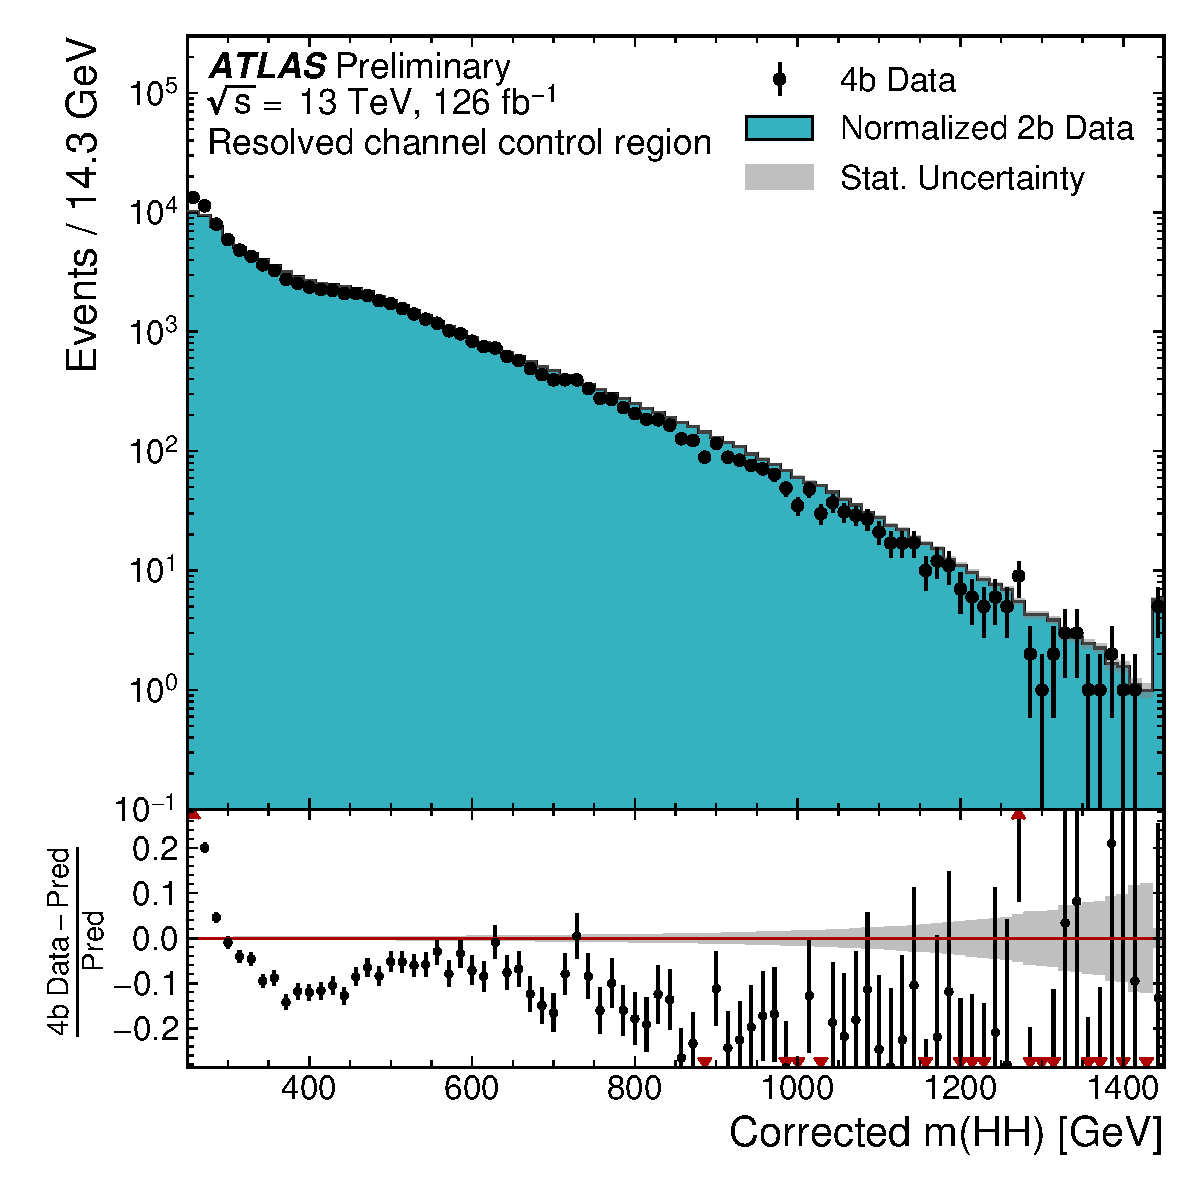
\includegraphics[width=0.48\textwidth]{figures/resolved-mhhcorr-cr-norw.pdf}
  }
  \subfloat[After Reweighting]{
    \label{fig:res-cr-rw}
    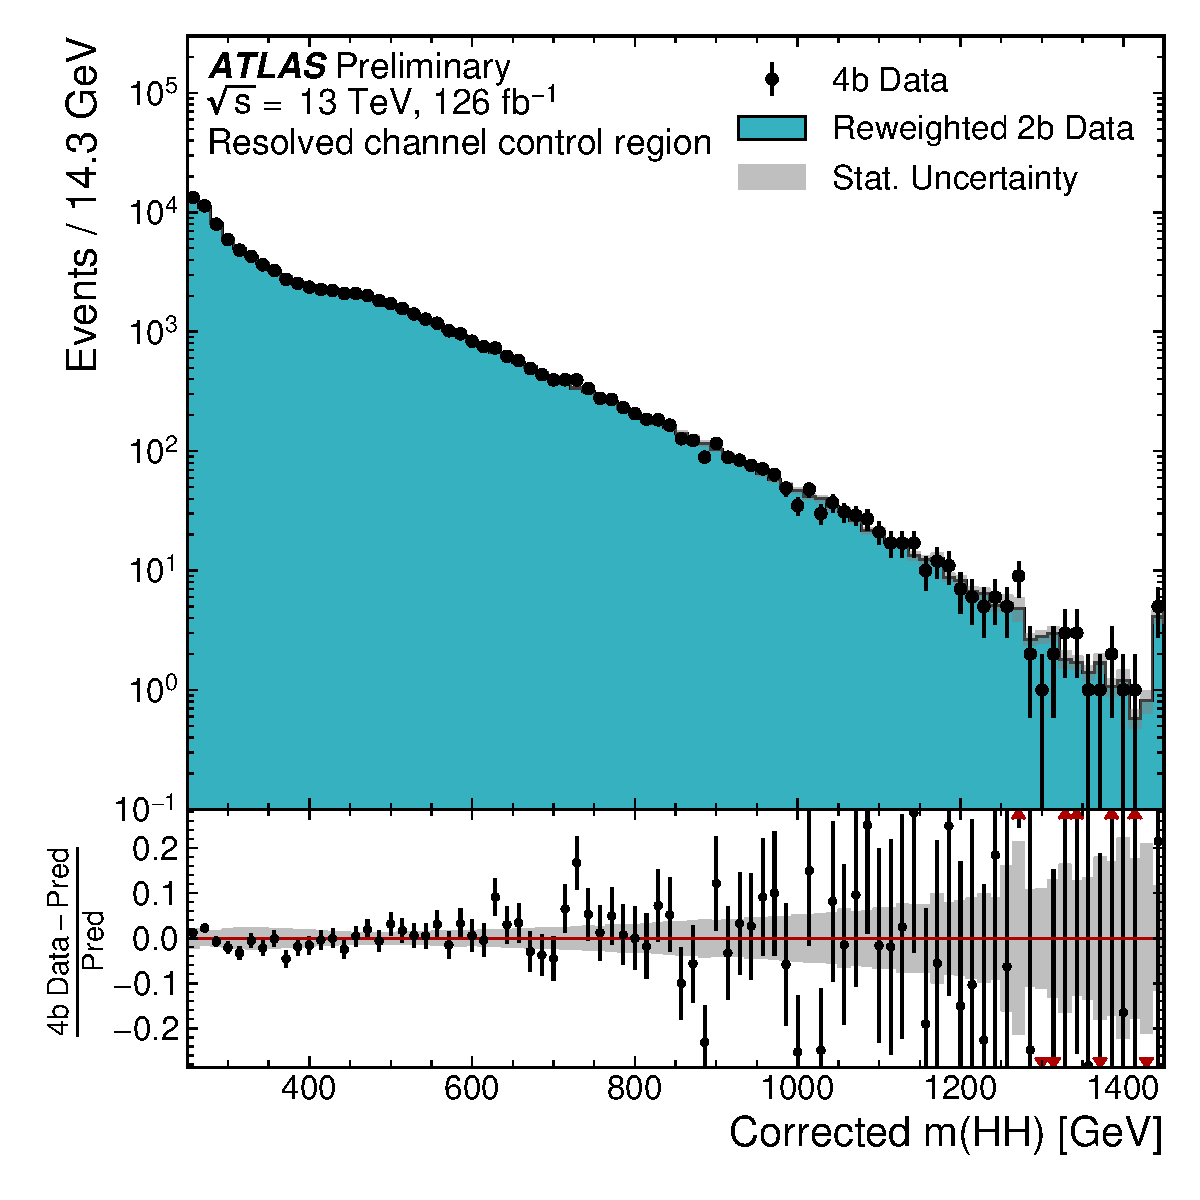
\includegraphics[width=0.48\textwidth]{figures/resolved-mhhcorr-cr-rw.pdf}
  }
  \caption{\label{fig:res-cr-mhh} \textbf{Resonant Search}: Demonstration of the performance of the nominal 
  reweighting in the control region on corrected $m_{HH}$, with Figure \ref{fig:res-cr-norw} showing 
  $2b$ events normalized to the total $4b$ yield and Figure \ref{fig:res-cr-rw} applying the 
  reweighting procedure. Agreement is much improved with the reweighting. Note that overall 
  reweighted $2b$ yield agrees with $4b$ yield in the control region by construction.}
\end{figure}

\begin{figure}[ht]
  \centering
  \subfloat{
    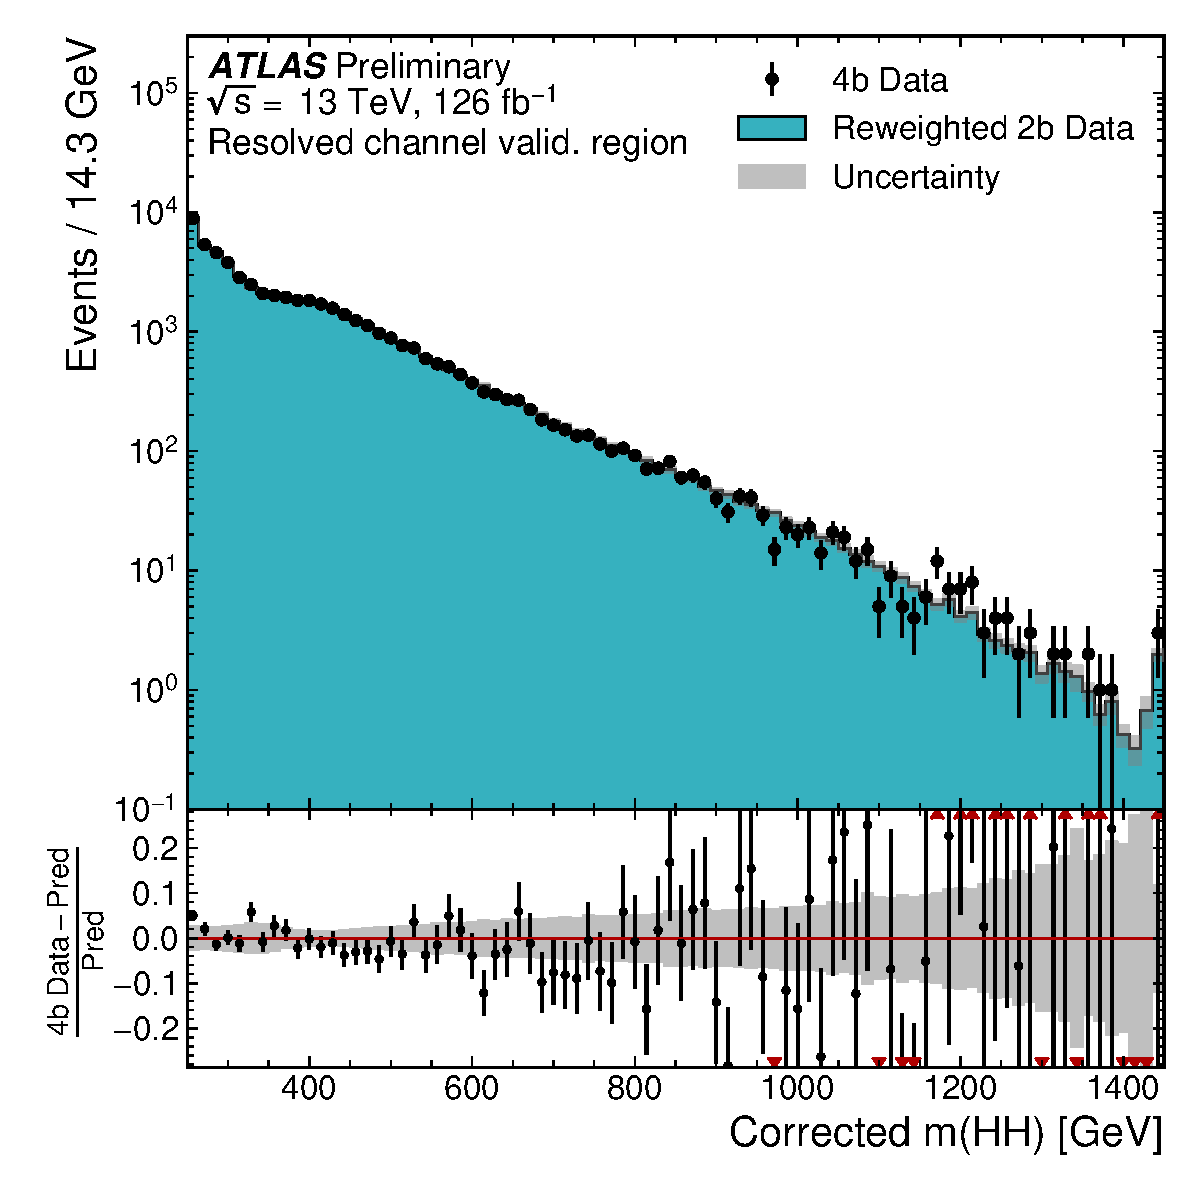
\includegraphics[width=0.65\textwidth]{figures/resolved-vr-mhh.pdf}
  }
  \caption{\label{fig:res-vr-mhh} \textbf{Resonant Search}: Demonstration of the performance 
  of the control region derived reweighting in the validation region on corrected $m_{HH}$. Agreement 
  is generally good for this extrapolated estimate. Note that the uncertainty band includes the 
  extrapolation systematic, which is defined by a reweighting trained in the validation region.}
\end{figure}

\begin{figure}[ht]
  \centering
  \subfloat{
    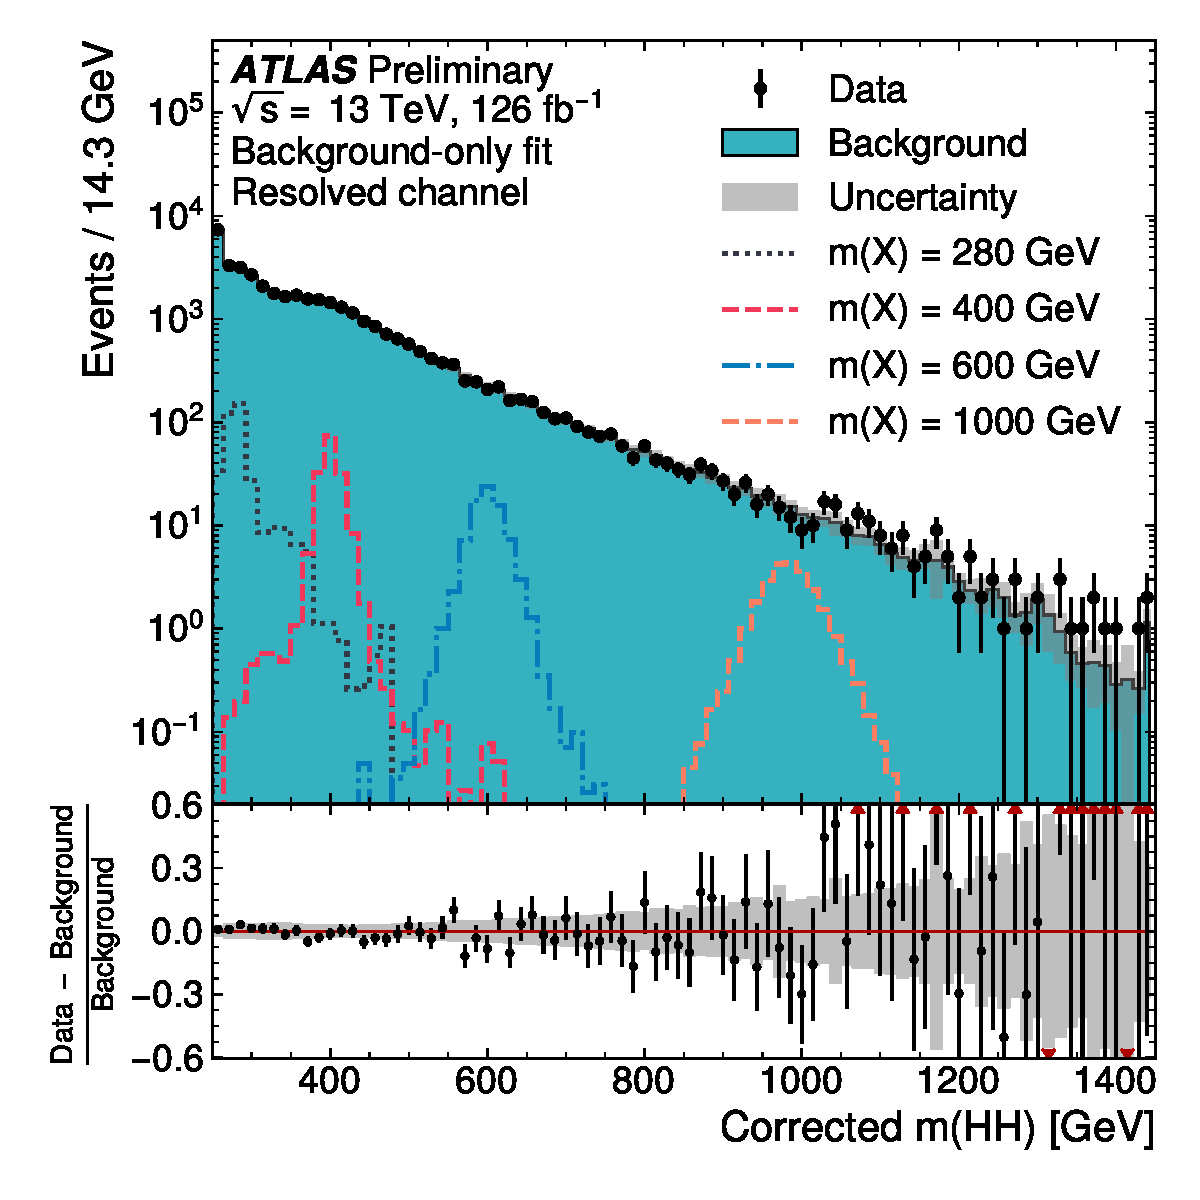
\includegraphics[width=0.48\textwidth]{figures/resolved-mhh.pdf}
  }
  \subfloat{
    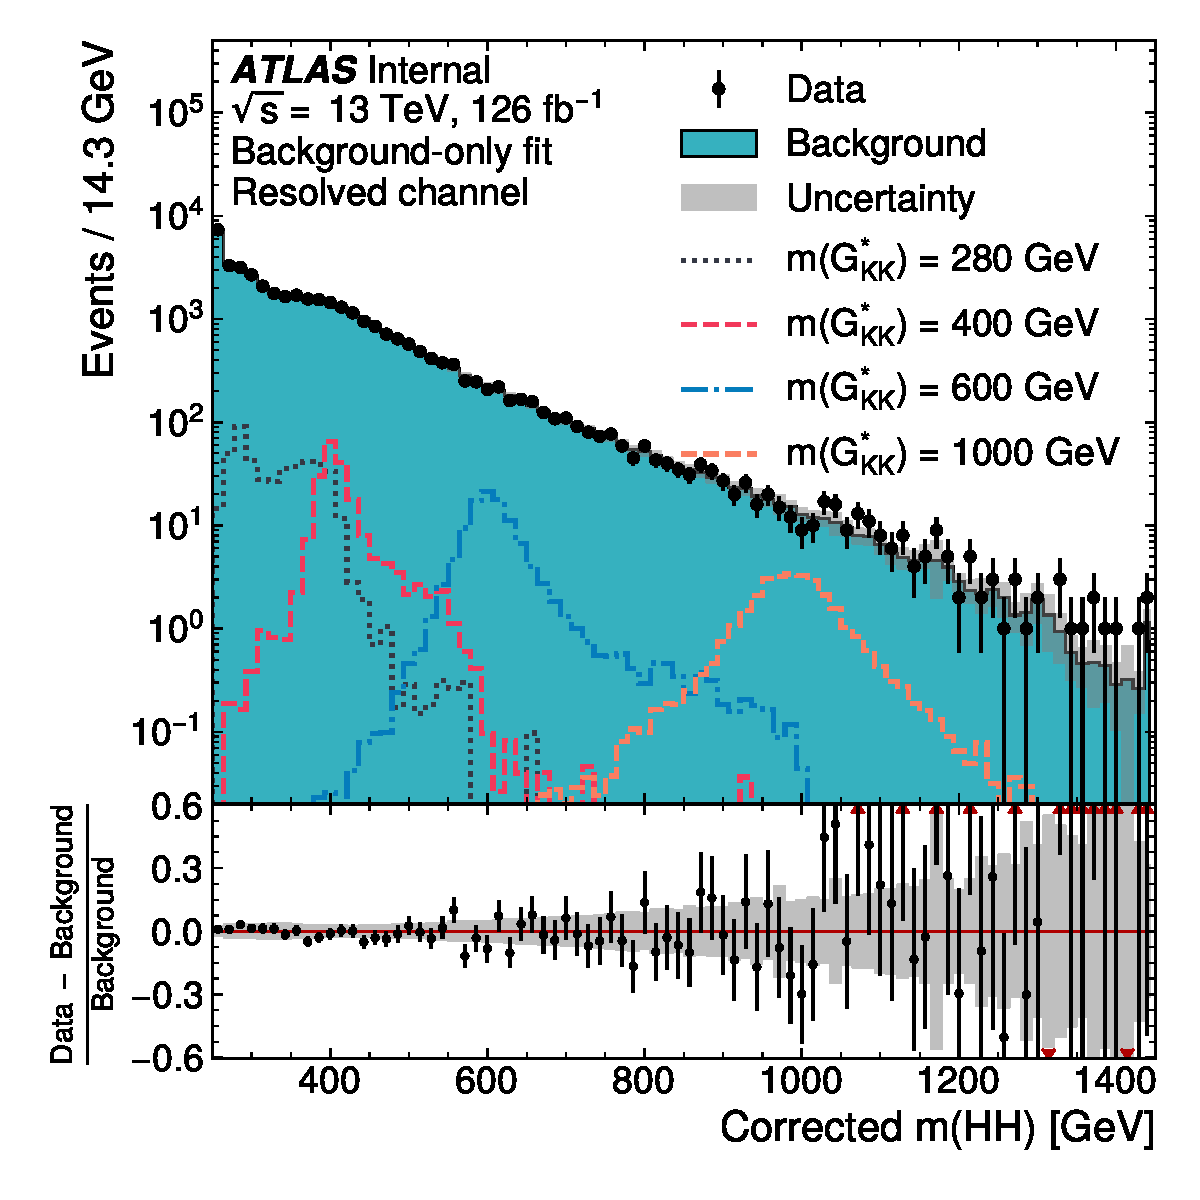
\includegraphics[width=0.48\textwidth]{figures/resolved-mhh-spin2.pdf}
  }
  \caption{\label{fig:res-sr-mhh} \textbf{Resonant Search}: Signal region agreement of the background estimate and 
  observed data after a background-only profile likelihood fit. The left plot overlays a variety of representative 
  spin-0 signals, while the right does the same for spin-2. The background and data are identical between the two. 
  The closure is generally quite good, though there is an evident deficit in the background estimate relative to the 
  data for higher values of corrected $m_{HH}$. Note that the spin-2 signals are significantly wider than the spin-0 
  signals. Near the kinematic threshold of \SI{250}{\GeV}, this leads to, e.g., the double peaked structure of the 
  \SI{280}{\GeV} signal, which is understood to be an effect of the limited kinematic phase space in this region.}
\end{figure}

\begin{table}[tbp]
  \begin{center}
    \caption{Resolved \(4b\) signal region data, estimated background, and signal event yields in corrected \mhh windows containing roughly 90\% of each signal, for representative spin-0 mass hypotheses.
             The signal is normalized to the overall expected limit on its cross-section; its uncertainties are evaluated by adding all individual components in quadrature.
             The background yields and uncertainties are evaluated after a background-only fit to the data. ~\cite{ATLAS-CONF-2021-035}.
            }
    \label{tab:resolved-yields-spin0}
    \sisetup{group-minimum-digits=4}
    \begin{tabular}{lc S[table-format=5.0] S[table-format=5.1]@{\(\;\pm\;\)}S[table-format=3.1] S[table-format=3.2]@{\(\;\pm\;\)}S[table-format=2.2]}
      \toprule
      \(m(X)\) [\GeV] & Corrected \mhh range [\GeV] & \multicolumn{1}{c}{Data}  & \multicolumn{2}{c}{Background model} & \multicolumn{2}{c}{Spin-0 signal model} \\ 
      \midrule
      260  &   [250, 321] & 18554 & 18300   & 110   & 503   & 43 \\
      500  &   [464, 536] &  2827 &  2866   &  22   & 105.4 & 5.7 \\
      800  &   [750, 850] &   358 &   366.2 &   7.3 &  37.7 & 1.7 \\
      1200 & [1079, 1250] &    68 &    52.6 &   1.7 &  11.71 & 0.62 \\
      \bottomrule
    \end{tabular}
  \end{center}
\end{table}

\begin{table}[tbp]
  \begin{center}
    \caption{Resolved \(4b\) signal region data, estimated background, and signal event yields in corrected \mhh windows containing roughly 90\% of each signal, for representative spin-2 mass hypotheses.
             The signal is normalized to the overall expected limit on its cross-section; its uncertainties are evaluated by adding all individual components in quadrature.
             The background yields and uncertainties are evaluated after a background-only fit to the data. ~\cite{ATLAS-CONF-2021-035}.
            }
    \label{tab:resolved-yields-spin2}
    \sisetup{group-minimum-digits=4}
    \begin{tabular}{lc S[table-format=5.0] S[table-format=5.1]@{\(\;\pm\;\)}S[table-format=3.1] S[table-format=3.2]@{\(\;\pm\;\)}S[table-format=2.2]}
      \toprule
      \(m(G_{KK}^{*})\) [\GeV] & Corrected \mhh range [\GeV] & \multicolumn{1}{c}{Data}  & \multicolumn{2}{c}{Background model} & \multicolumn{2}{c}{Spin-2 signal model} \\ 
      \midrule
      260  &  [250, 393] & 26775 & 26650   & 130   & 368    & 25 \\
      500  &  [464, 636] &  4655 &  4719   &  37   & 138.6  &  5.7 \\
      800  &  [707, 950] &   795 &   811   &  13   &  52.1  &  1.9 \\
      1200 & [993, 1279] &   146 &   120.6 &   2.8 &  14.45 &  0.67 \\
      \bottomrule
    \end{tabular}
  \end{center}
\end{table}


\FloatBarrier
\subsection{Non-resonant Search}
As discussed above, the non-resonant search splits the signal extraction into two categories of 
$\Delta\eta_{HH}$ ($0 \leq \Delta\eta_{HH} < 0.75$ and $0.75 \leq \Delta\eta_{HH} < 1.5$), 
and two categories of $X_{HH}$ ($0 \leq X_{HH} < 0.95$ and $0.95 \leq X_{HH} < 1.6$). 
To maintain reasonable statistics in each bin entering the signal extraction fit, a 
variable width binning is considered defined by a resolution parameter, $r$, and a set range in 
$m_{HH}$, where bin edges are determined iteratively as
\begin{equation}
b_{low}^{i+1} = b_{low}^{i} + r\cdot b_{low}^{i},
\end{equation}
where $b_{low}^{i}$ is the low edge of bin $i$. The parameters used here are 
$r=0.08$ over a range from \SI{280}{\GeV} to \SI{975}{\GeV}, and underflow and 
overflow are included in the initial and final bin contents respectively. $m_{HH}$ with 
no correction is used as the final discriminant in each category.

A demonstration of the performance of the reweighting on distributions unrolled across categories is shown 
in Figures \ref{fig:nonres-4b-CR} and \ref{fig:nonres-3b1l-CR} for the control region and 
Figures \ref{fig:nonres-4b-VR} and \ref{fig:nonres-3b1l-VR} for 
the validation region. A background-only profile likelihood fit is run for the distribution in the signal 
region, and results with the Standard Model $HH$ signal and $\kappa_{\lambda}=6$ signal overlaid are shown for $4b$ in Figure \ref{fig:nonres-sr-mhh-4b} and $3b1l$ in Figure \ref{fig:nonres-sr-mhh-3b1l}. Note that 
the plots show the sum across all years, but the signal extraction fit and background estimate are run with the 
years separately. All bins are normalized to represent a density of Events / \SI{15}{\GeV}.

\begin{figure}[ht]
  \centering
  \subfloat{
    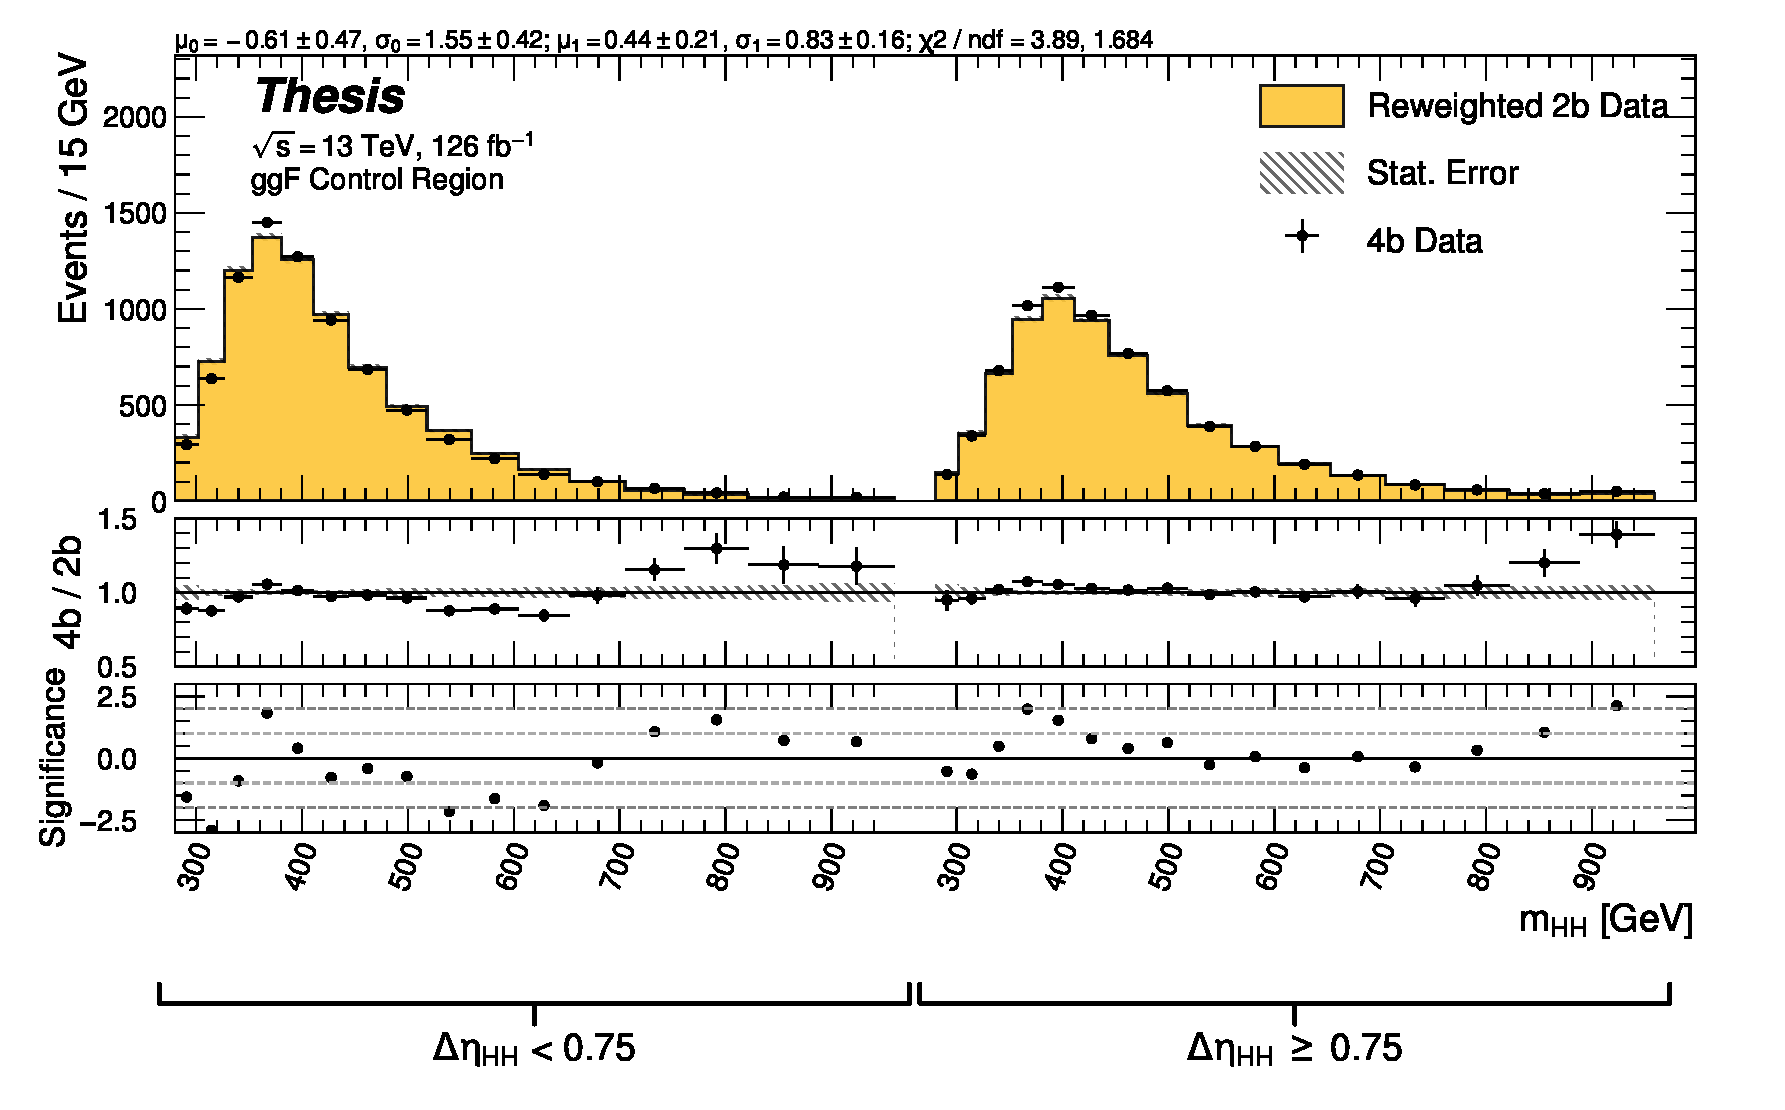
\includegraphics[width=1.0\textwidth]{figures/nonres-4b-CR.pdf}
  }
  \caption{\label{fig:nonres-4b-CR} \textbf{Non-resonant Search (4b)}: Demonstration of the performance of the nominal reweighting in the control region on $m_{HH}$, split into the two $\Delta\eta_{HH}$ regions. Closure is generally good, 
  with some residual mis-modeling in the low $\Delta\eta_{HH}$ region near \SI{600}{\GeV}.}
\end{figure}

\begin{figure}[ht]
  \centering
  \subfloat{
    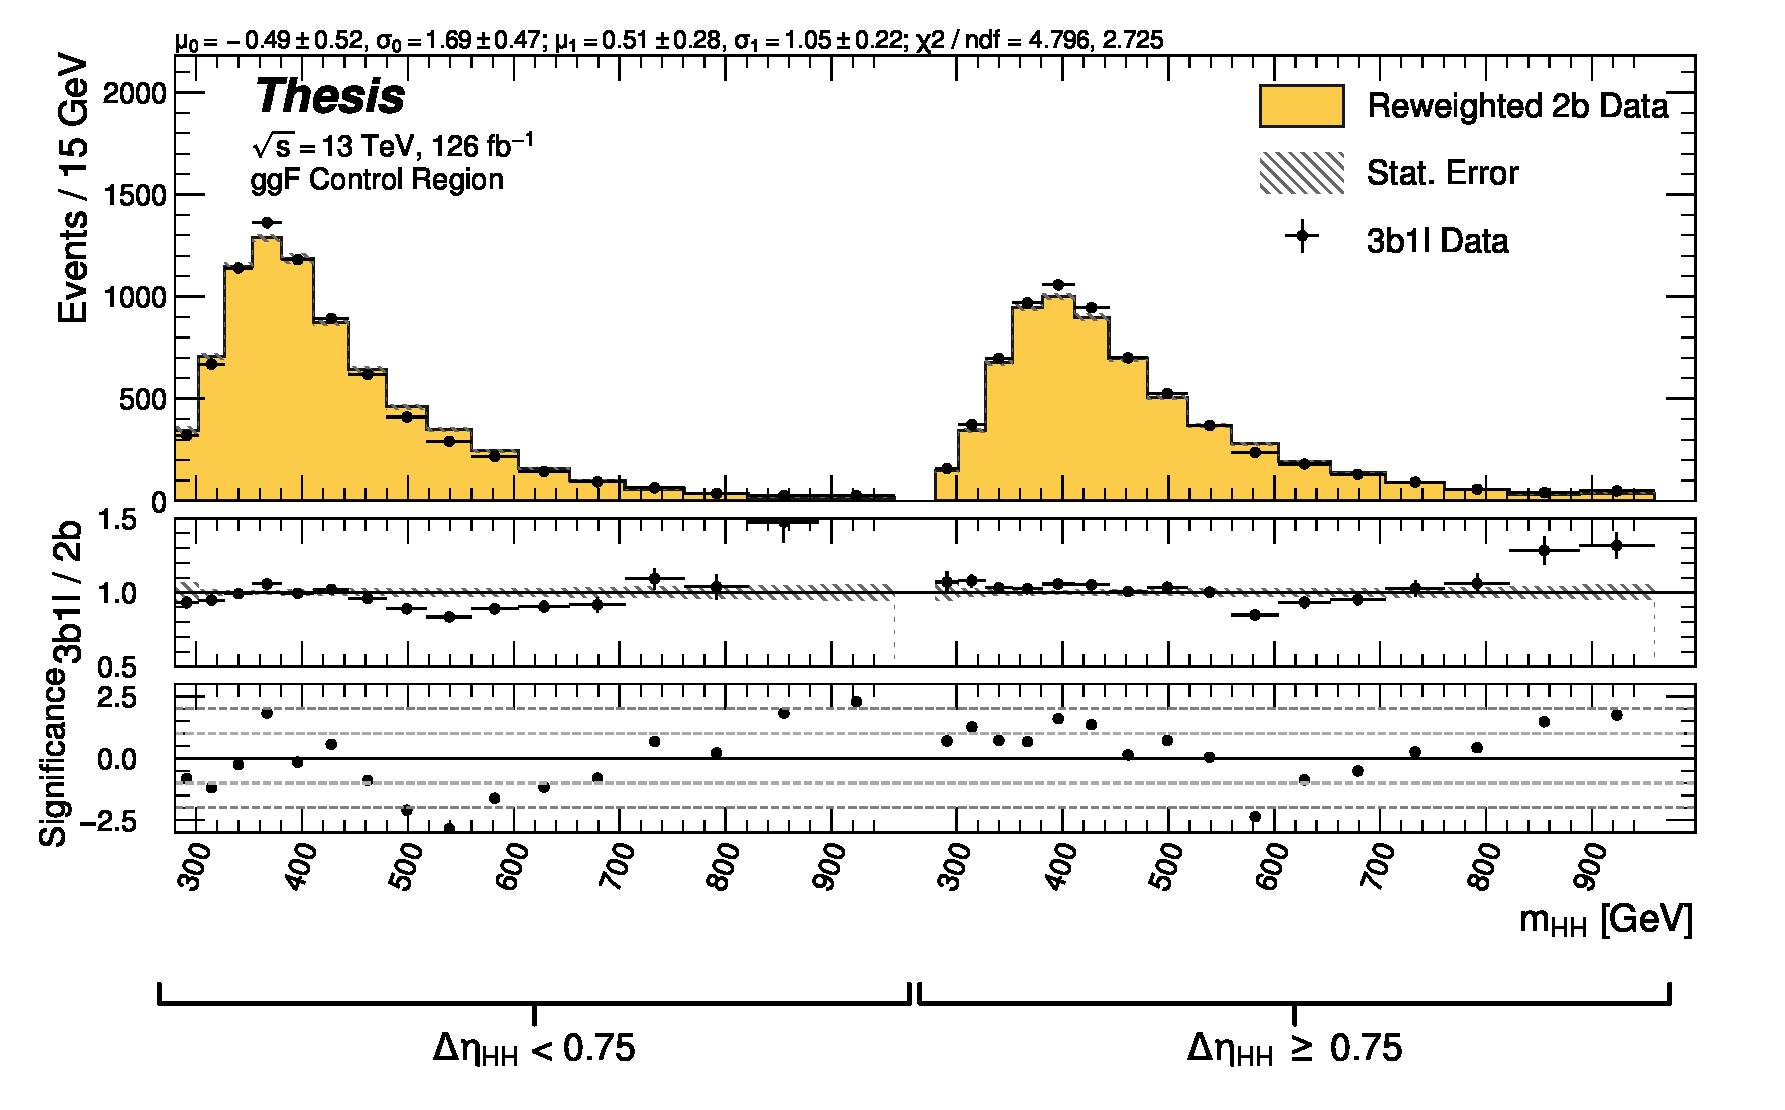
\includegraphics[width=1.0\textwidth]{figures/nonres-3b1l-CR.pdf}
  }
  \caption{\label{fig:nonres-3b1l-CR} \textbf{Non-resonant Search (3b1l)}: Demonstration of the performance of the nominal reweighting in the control region on $m_{HH}$, split into the two $\Delta\eta_{HH}$ regions. Closure is generally good, with similar conclusions as for the $4b$ region.}
\end{figure}

\begin{figure}[ht]
  \centering
  \subfloat{
    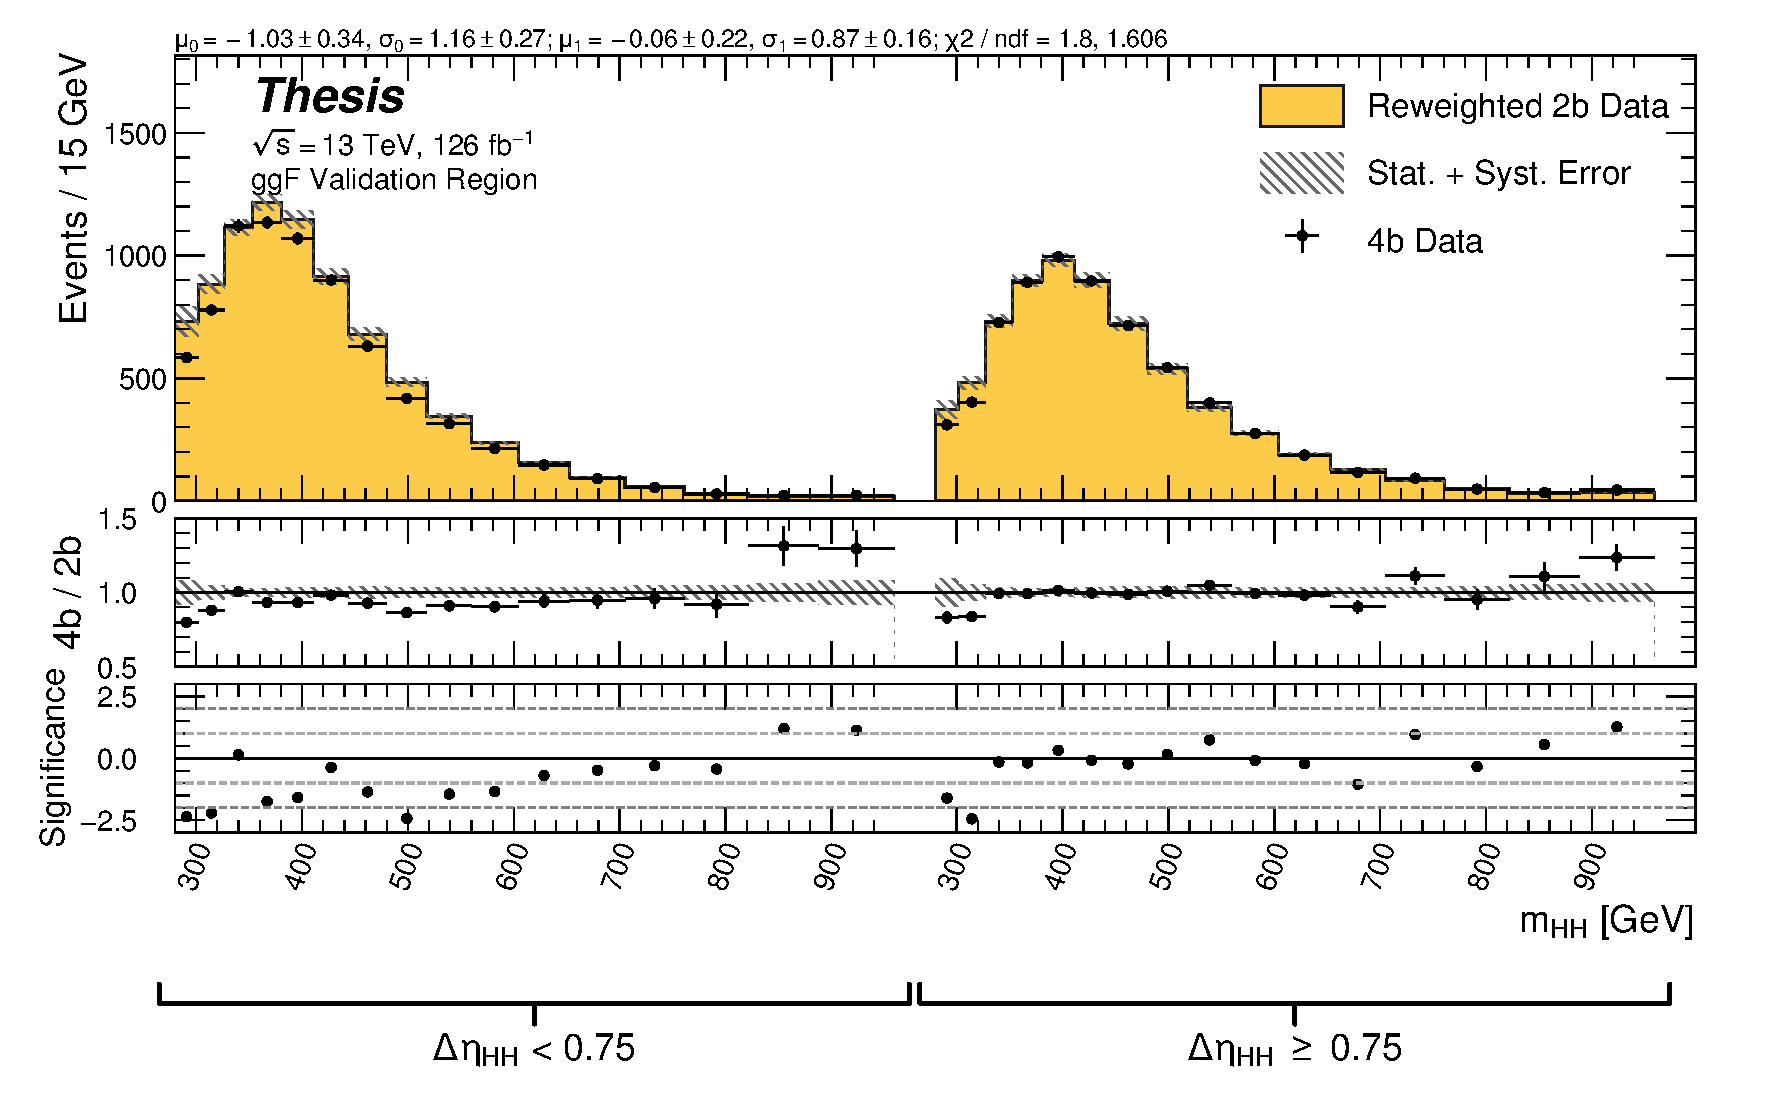
\includegraphics[width=1.0\textwidth]{figures/nonres-4b-VR.pdf}
  }
  \caption{\label{fig:nonres-4b-VR} \textbf{Non-resonant Search (4b)}: Demonstration of the performance of the nominal reweighting in the validation region on $m_{HH}$, split into the two $\Delta\eta_{HH}$ regions. The low $\Delta\eta_{HH}$ region is consistently overestimated, but, systematic uncertainties are defined via the difference between 
  VR and CR estimates.}
\end{figure}

\begin{figure}[ht]
  \centering
  \subfloat{
    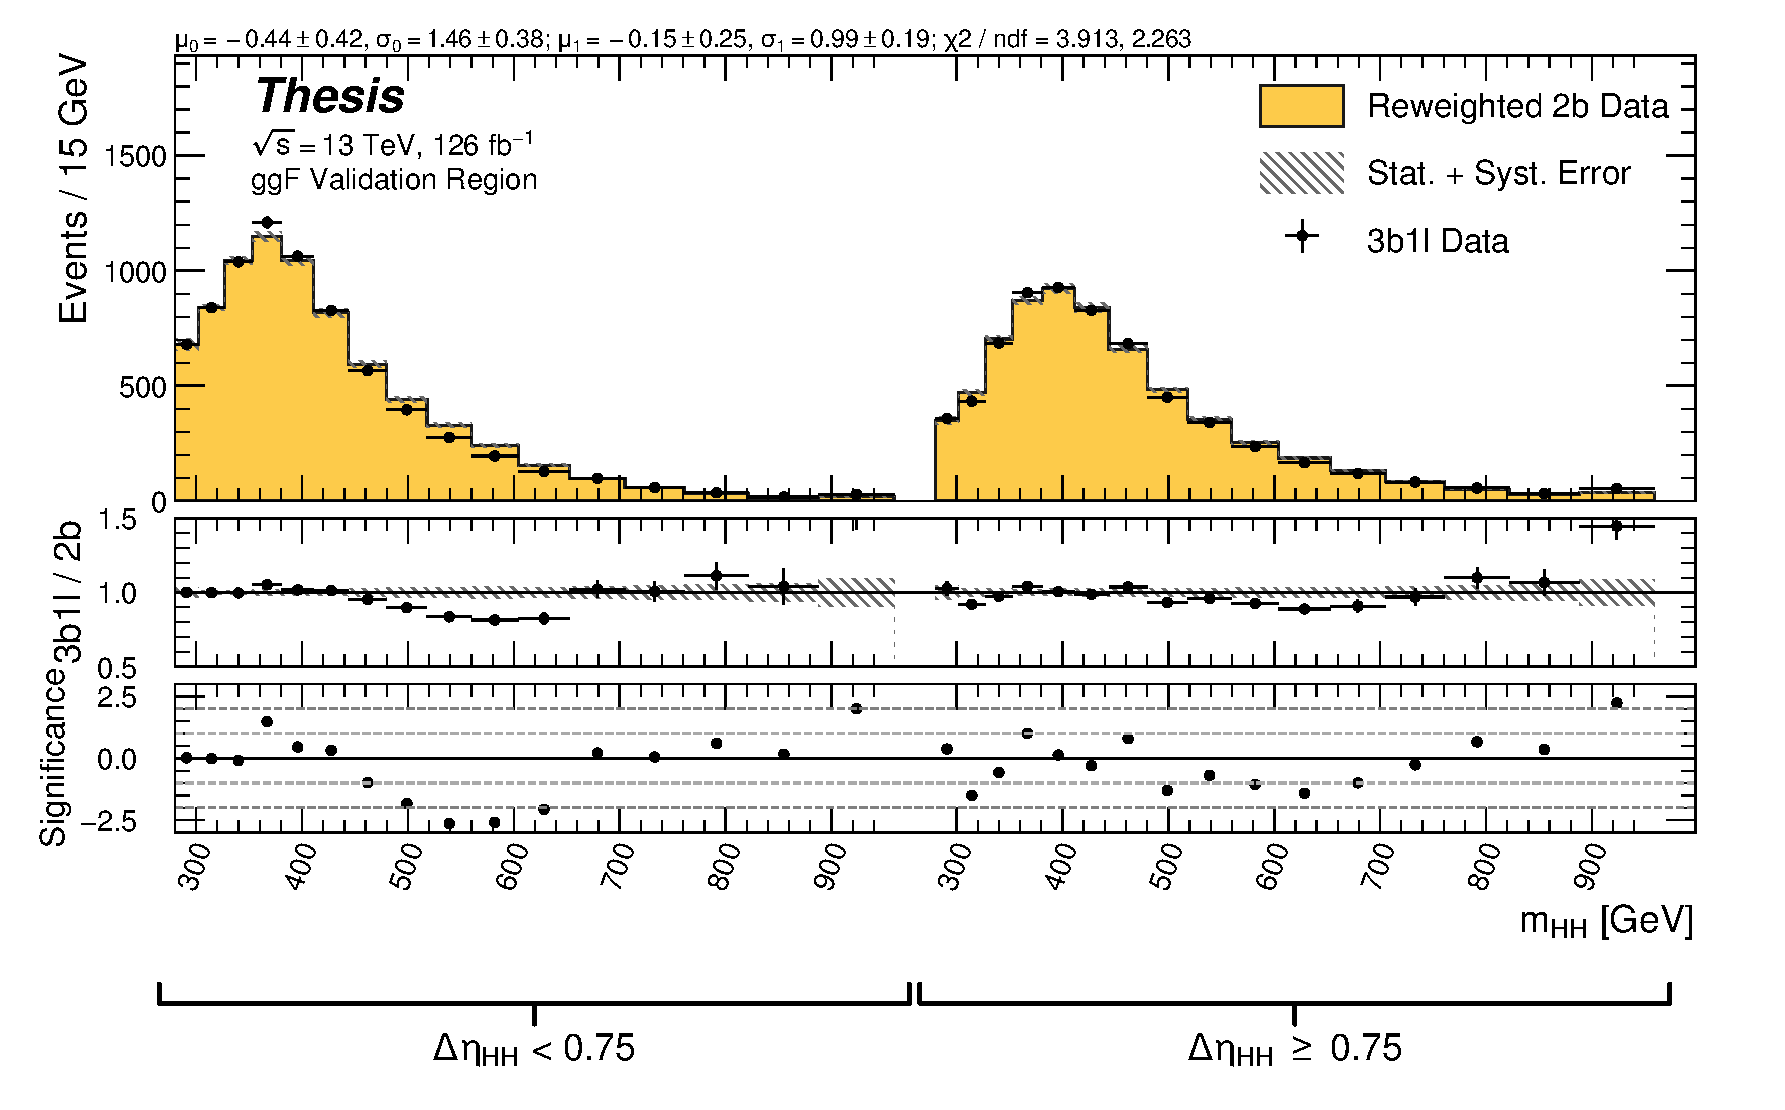
\includegraphics[width=1.0\textwidth]{figures/nonres-3b1l-VR.pdf}
  }
  \caption{\label{fig:nonres-3b1l-VR} \textbf{Non-resonant Search (3b1l)}: Demonstration of the performance of the nominal reweighting in the validation region on $m_{HH}$, split into the two $\Delta\eta_{HH}$ regions. A deficit 
  is present near \SI{600}{\GeV}, but agreement is fairly good otherwise.}
\end{figure}


\begin{figure}[ht]
  \centering
  \hspace*{-2cm}
  \subfloat{
    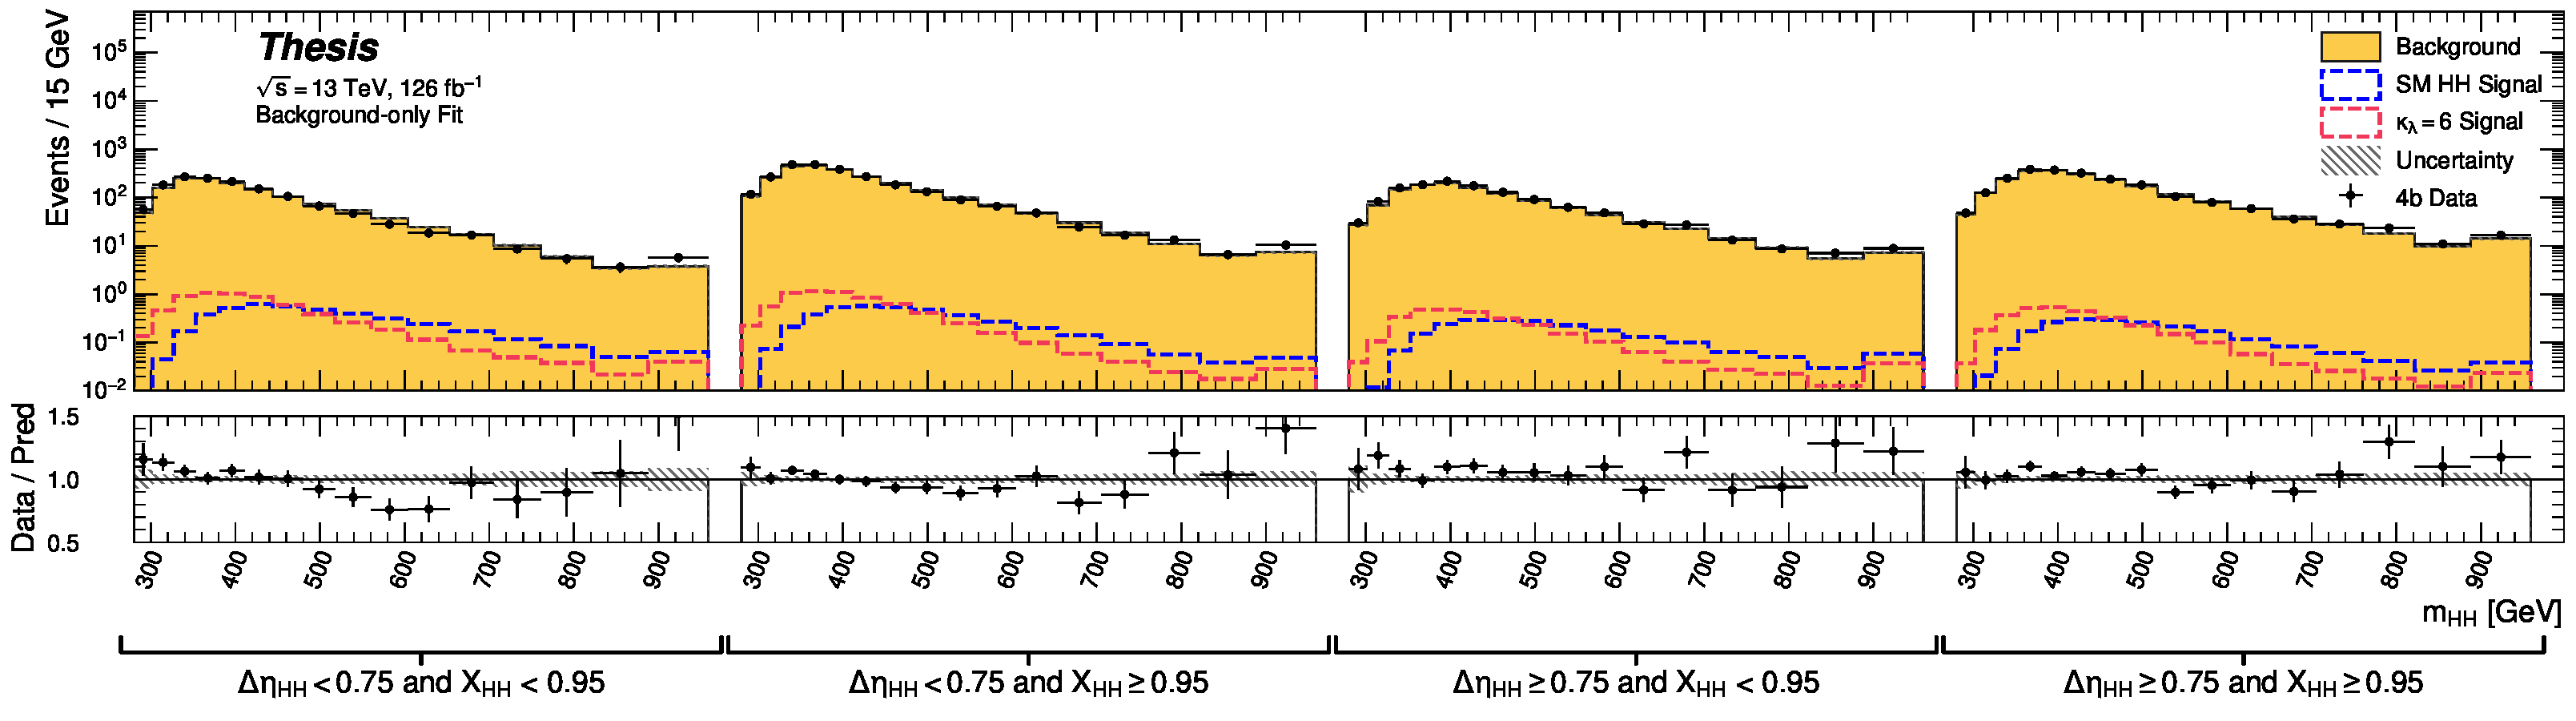
\includegraphics[width=1.2\textwidth]{figures/post-bonly-fit-4b-nonres-with-SM-HH-and-kl-6.pdf}
  }
  \caption{\label{fig:nonres-sr-mhh-4b} \textbf{Non-resonant Search (4b)}: Signal region agreement of the background estimate and observed data after a background-only profile likelihood fit for the $4b$ channels, with Standard Model 
  and $\kappa_{\lambda}=6$ signal overlaid for reference. Modeling is generally quite good near the Standard Model peak, but disagreements are seen at very low and high masses. A deficit is present in low $\Delta\eta_{HH}$ bins near \SI{600}{\GeV}.}
\end{figure}

\begin{figure}[ht]
  \centering
   \hspace*{-2cm}
  \subfloat{
    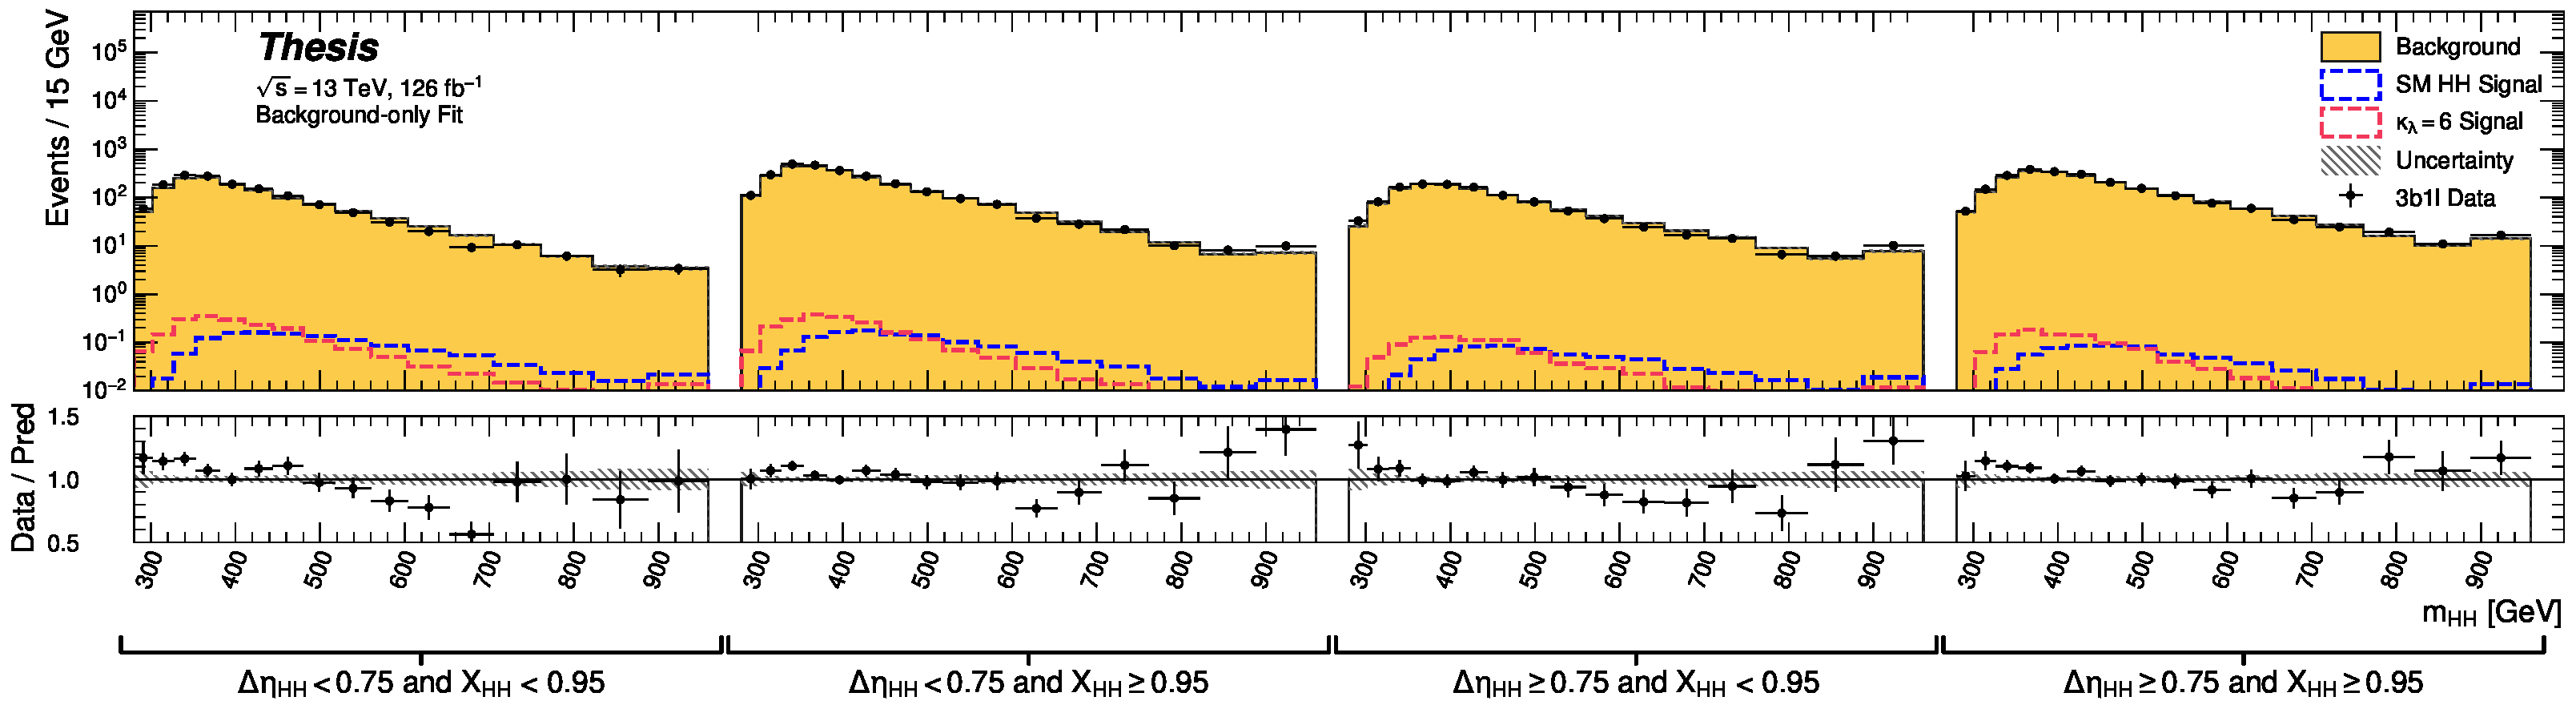
\includegraphics[width=1.2\textwidth]{figures/post-bonly-fit-3b1l-nonres-with-SM-HH-and-kl-6.pdf}
  }
  \caption{\label{fig:nonres-sr-mhh-3b1l} \textbf{Non-resonant Search (3b1l)}: Signal region agreement of the background estimate and observed data after a background-only profile likelihood fit for the $3b1l$ channels, with Standard Model
  and $\kappa_{\lambda}=6$ signal overlaid for reference. Conclusions are very similar to the $4b$ channels, with generally good modeling near he Standard Model peak, but disagreements at very low and high masses. A deficit is present near \SI{600}{\GeV}.}
\end{figure}

\FloatBarrier
\clearpage
\section{Statistical Analysis}
The resonant analysis is used to set a 95\% confidence level upper limit on the
\HepProcess{\Pp \Pp \to \PScal \to \higgs \higgs \to \Pqb \Paqb \Pqb \Paqb} and
\HepProcess{\Pp \Pp \to \PGrav \to \higgs \higgs \to \Pqb \Paqb \Pqb \Paqb} cross-sections, 
while the non-resonant analysis is used to set a 95\% confidence level upper limit on the
\HepProcess{\Pp \Pp \to \higgs \higgs \to \Pqb \Paqb \Pqb \Paqb} cross sections for a 
variety of values of the trilinear Higgs coupling.

The upper limit is extracted using the \CLs method \cite{Read02}. The test statistic 
used is \qmu \cite{Cowan11}, where $\mu$ is the signal strength, and $\mathbf{\theta}$ represents the nuisance
parameters. A single hat represents
the maximum likelihood estimate of a parameter, while
$\doublehat{\mathbf{\theta}}\qty(x)$ represents the conditional maximum
likelihood estimate of the nuisance parameters if the signal cross-section is
fixed at $x$.


\begin{equation}
	\label{eqn:qmu-def}
	\qmu =
	\begin{cases}
		-2\ln(\frac{\lhood\qty(\mu, \doublehat{\mathbf{\theta}}\qty(\mu))}{\lhood\qty(\hat{\mu},
		\hat{\mathbf{\theta}})})              & \hat{\mu} \le \mu \\
		0                                     & \hat{\mu} > \mu
	\end{cases}
\end{equation}

\CLs for some test value of $\mu$ is then defined by

\begin{equation}
	\label{eqn:cls-def}
	\CLs = \frac{\CLsb}{\CLb} = \frac{p\qty(\qmu \ge \qmuobs | s + b)}{p\qty(\qmu \ge \qmuobs | b)},
\end{equation}

where the $p$-values are calculated in the asymptotic approximation
\cite{Cowan11}, which is valid in the large sample limit.

The signal cross-section {$\mu$}~\si{\femto\barn} is excluded at the 95\% confidence level if $\CLs < 0.05$.

Nuisance parameter pulls and impacts for the background extrapolation uncertainties are shown for representative scalar 
resonances in Figure \ref{fig:res-pull-imp}. Note that the fit includes all uncertainties. The $H_{T}$ nuisance 
parameters are significantly pulled, corresponding to the expectation that the resonant validation region is 
more similar to the signal region than the resonant control region is, though the control region is 
where the nominal estimate is derived. A variety of 
cross-checks have been done to confirm the healthy behavior of the signal extraction fit, despite these large pulls.
\begin{figure}[ht]
  \centering

  \subfloat{
    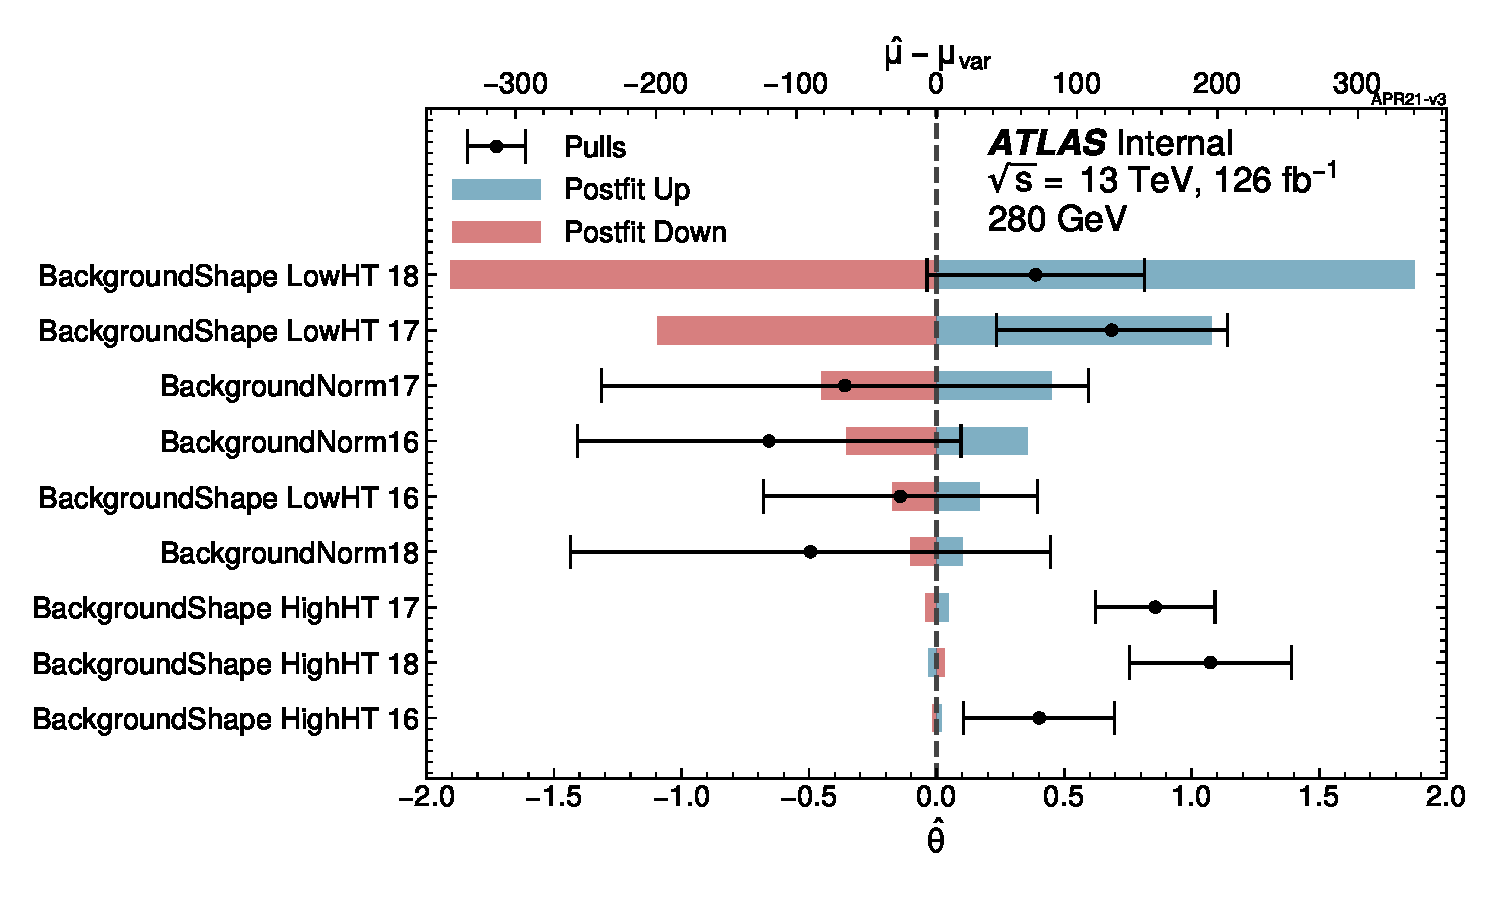
\includegraphics[width=0.48\textwidth]{figures/pulls-impacts-280}
  }
  \subfloat{
    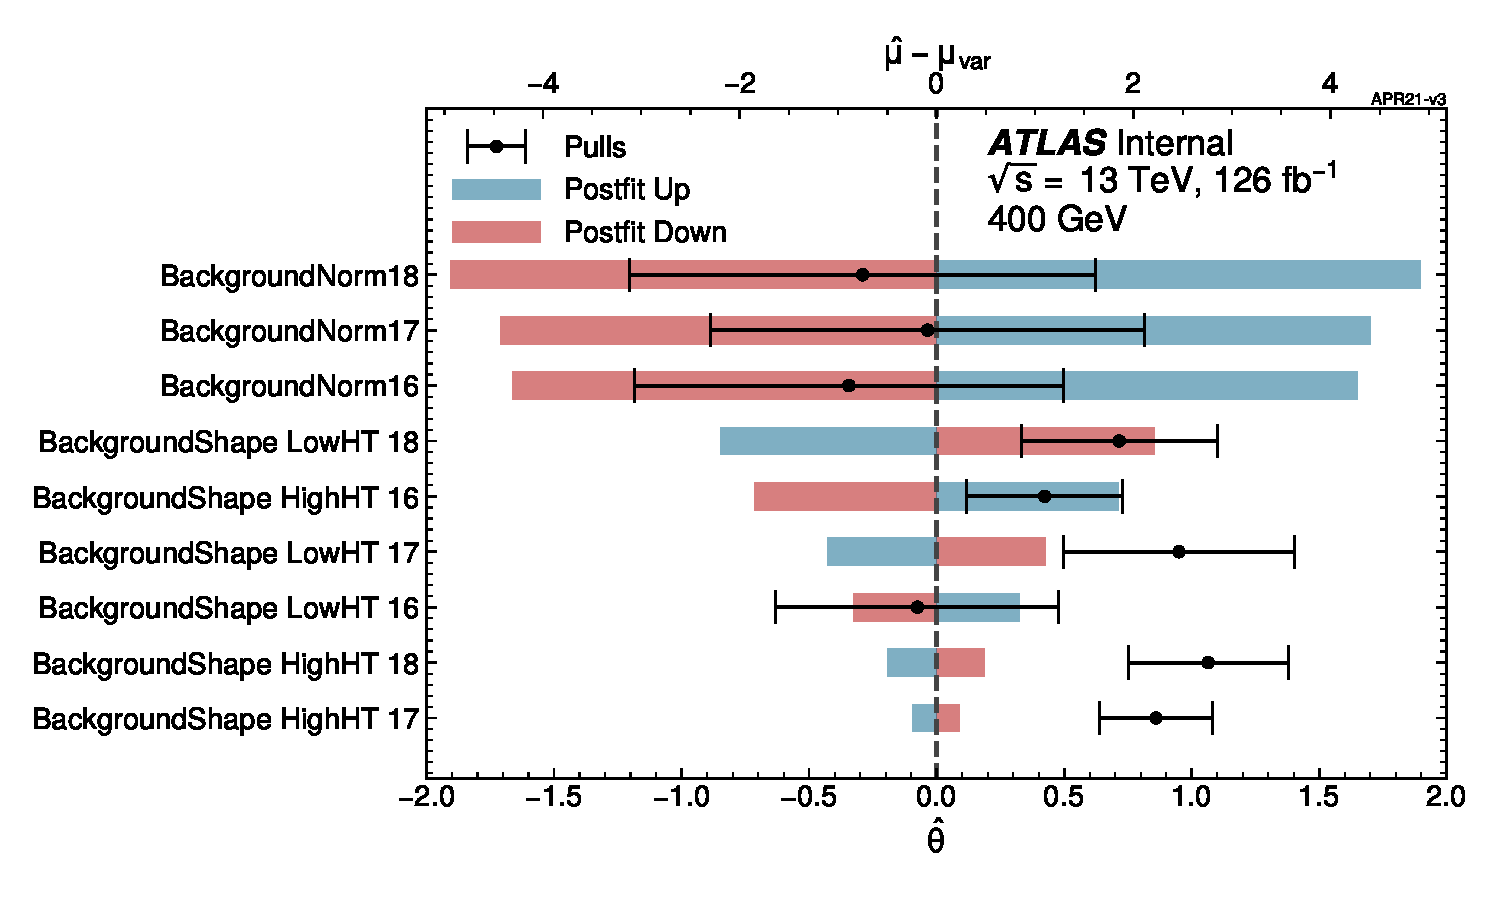
\includegraphics[width=0.48\textwidth]{figures/pulls-impacts-400}
  }

  \subfloat{
    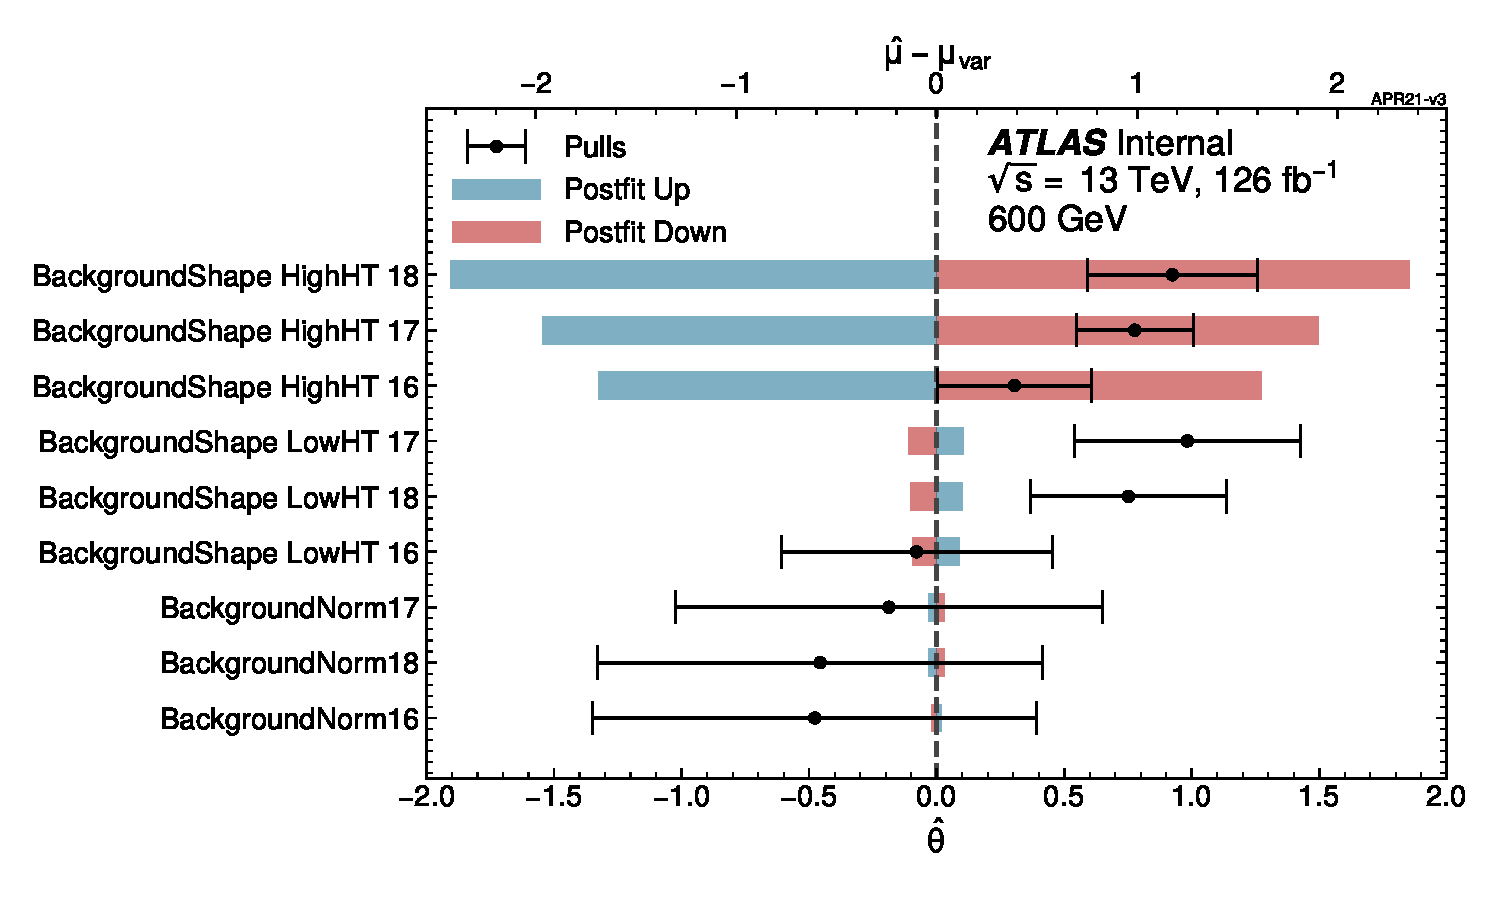
\includegraphics[width=0.48\textwidth]{figures/pulls-impacts-600}
  }
    \subfloat{
    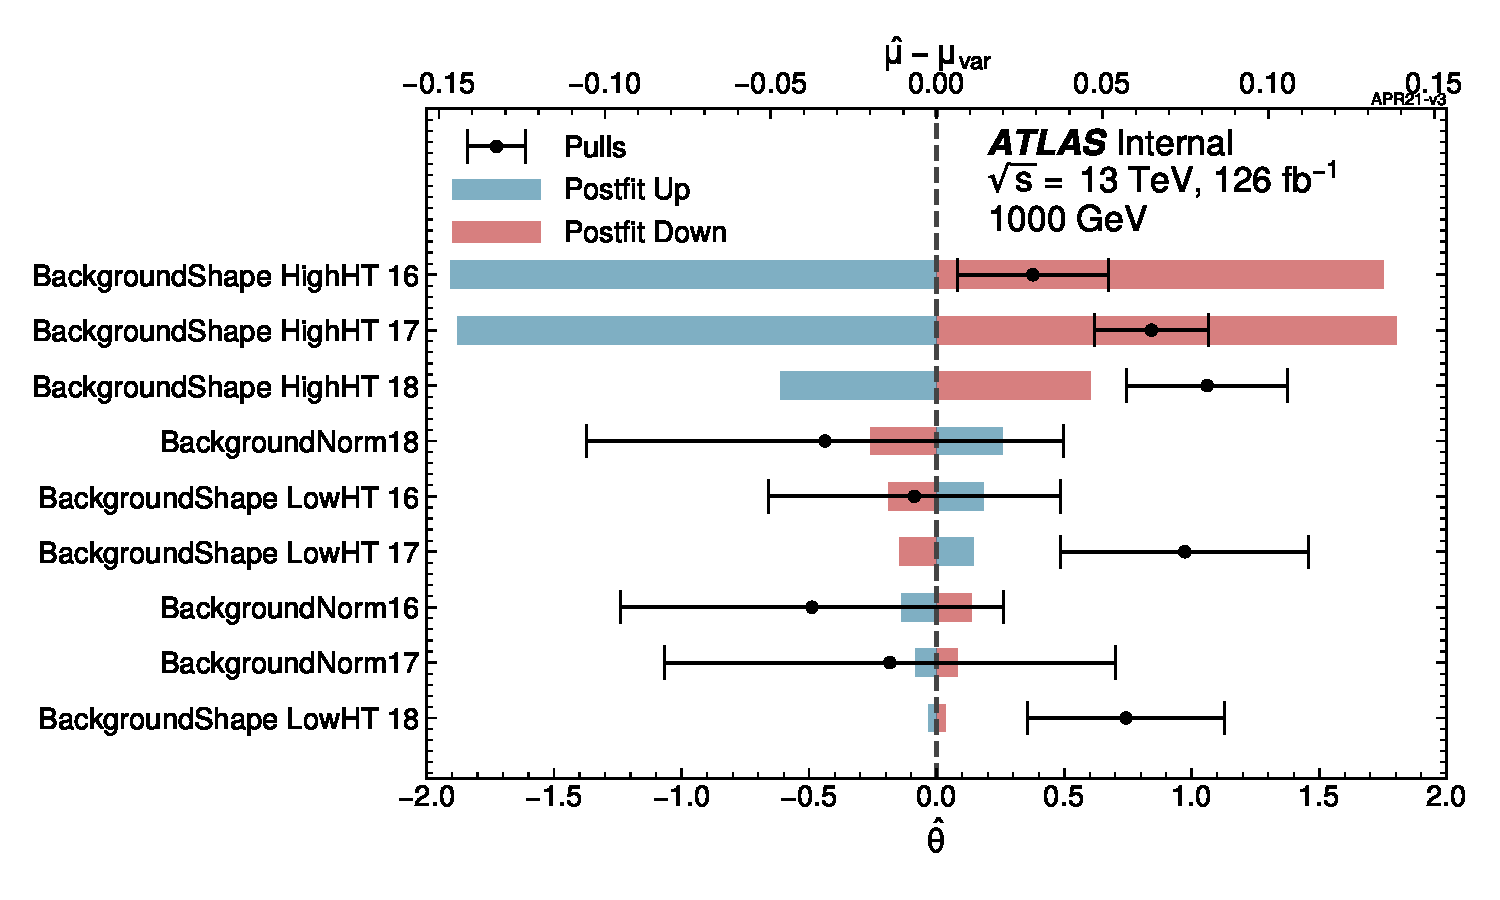
\includegraphics[width=0.48\textwidth]{figures/pulls-impacts-1000}
  }
  \caption{\label{fig:res-pull-imp} Pulls and impacts of the background extrapolation uncertainties for 
  the resonant analysis, ranked by magnitude of post-fit impact and shown for a variety of representative scalar 
  signals. Significant pulls of the $H_{T}$ systematics are present, corresponding to the expectation that the 
  validation region is more similar to the signal region than the control region is. Nuisance parameter pulls 
  are generally consistent across signal mass, but impacts vary, with low $H_{T}$ having the largest impact 
  for low mass, and high $H_{T}$ for high mass. \SI{400}{\GeV} is near the split between the two regimes.}
\end{figure}

Corresponding nuisance parameter pulls for the Standard Model non-resonant search are shown in 
Figure \ref{fig:nonres-pull}. There are significantly more parameters than the resonant search due to the 
category scheme, as well as due to the splitting of the control/validation region comparison systematic into 
four signal region quadrants. In general, however, the pulls are well behaved, and are generally consistent 
with 0. The largest deviating pulls are less constrained than in the resonant search, such that these 
deviations are still within $2\sigma$ of $0$.

\begin{figure}[ht]
  \centering
  \hspace*{-2cm}
  \subfloat{
    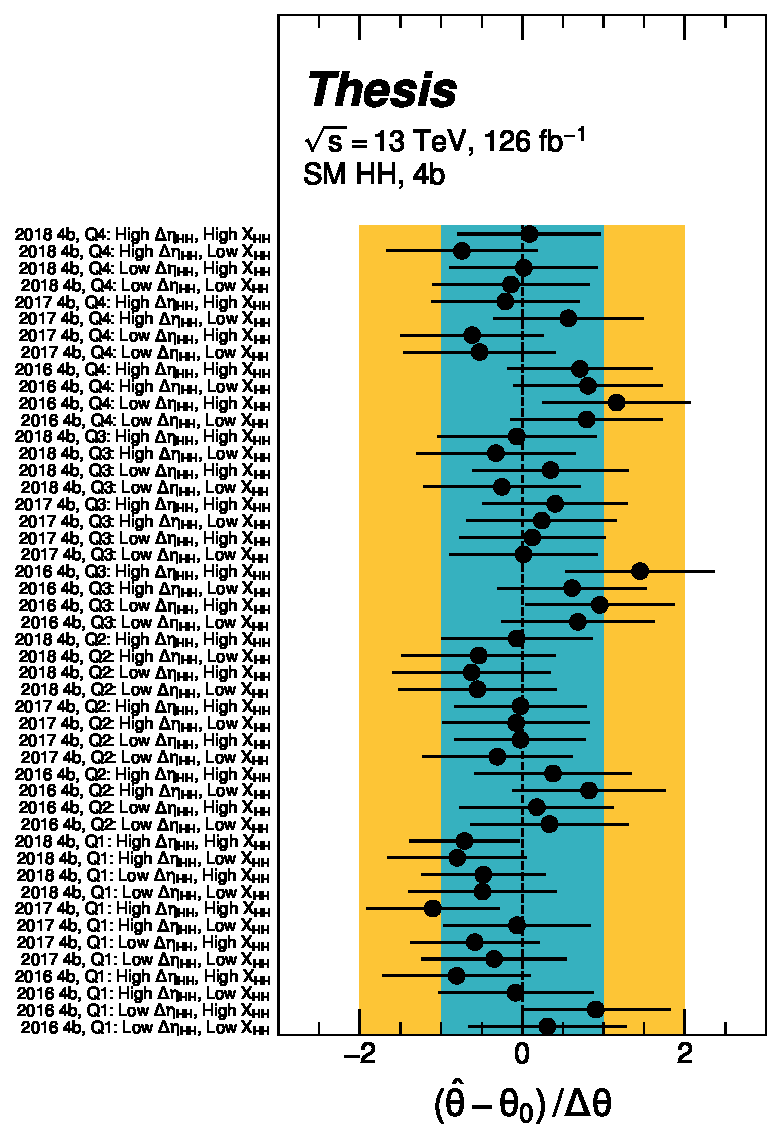
\includegraphics[width=0.48\textwidth]{figures/unb-pulls-SM-HH-4b}
  }
  \subfloat{
    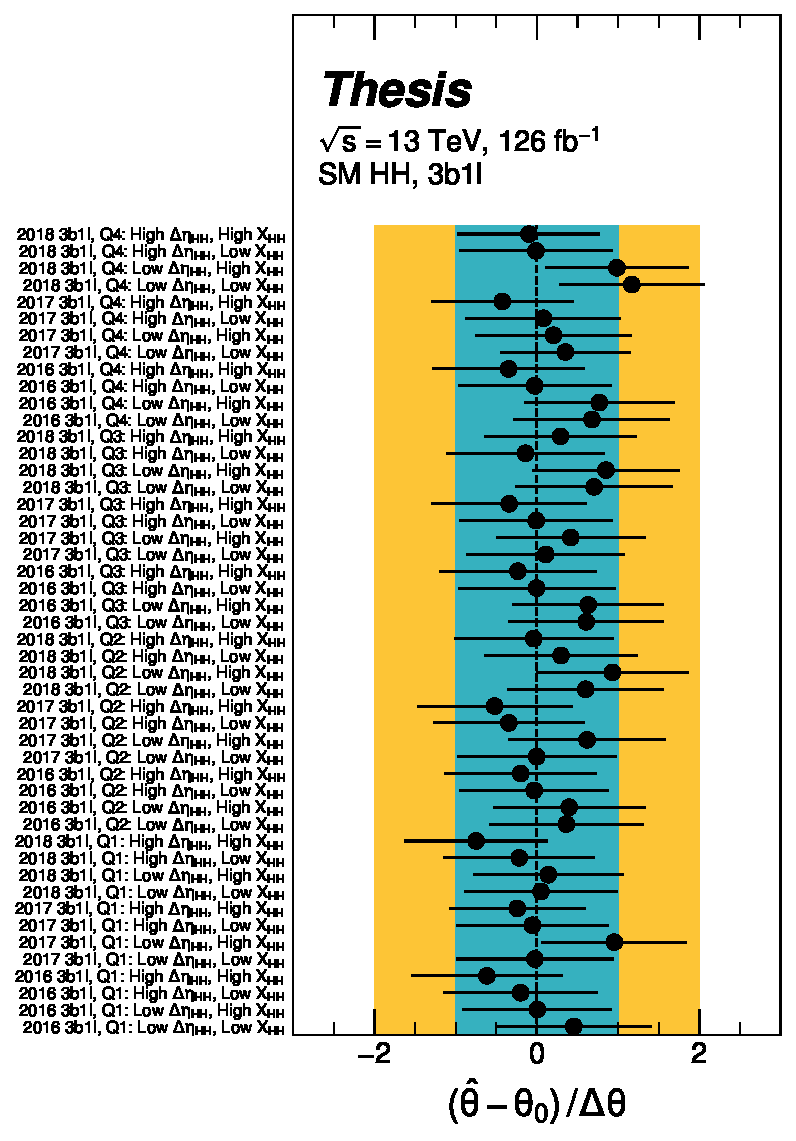
\includegraphics[width=0.49\textwidth]{figures/unb-pulls-SM-HH-3b1l}
  }

  \caption{\label{fig:nonres-pull} Background control/validation region systematic nuisance parameter pulls for 
  the Standard Model non-resonant signal, shown for $4b$ (left) and $3b1l$ (right) separately, though the two channels 
  are fit together. There are four signal region quadrant nuisance parameters for each category in the $2\times 2$ scheme 
  in $\Delta \eta_{HH}$ and $X_{HH}$, and each year is treated as a separate channel in the fit. Pulls are generally 
  consistent with zero, though there are some trends: quadrant 1 $4b$ tends to be pulled negatively, 2016 tends to 
  be pulled positively. Note that $4b$ dominates the sensitivity relative to $3b1l$.}
\end{figure}


\FloatBarrier
\clearpage
\section{Results}
Figure \ref{fig:res-limits} shows the expected limit for the spin-0 and spin-2 resonant search. The 
resolved channel covers the range between \SIlist{251;1500}{\GeV} and is combined with the boosted channel (see Appendix \ref{app:other-channels}) between 
\SIlist{900;1500}{\GeV}. The boosted channel then extends to \SI{5}{\TeV}. All results use the asymptotic approximation, 
though the validity of such an approximation for the boosted results above \SI{3}{\TeV} is being studied. 
The most significant excess is seen for a signal mass of \SI{1100}{\GeV}, with local significance of 
$2.6\sigma$ for the spin-0 signal and 
$2.7\sigma$ for the spin-2 signal. To account for the look-elsewhere effect, namely, the fact that the search is 
performed over many mass points rather than just one, a global significance is calculated following the procedure 
in~\cite{LookElsewhereEffect}. Pseudo-experiments are generated from a background-only model which has been fit to 
data. These are used to construct a distribution of local $p$-values as a function of resonance mass. The number of 
level crossings below a reference level of $p=0.5$ is used together with the local $p$-value 
to compute a global $p$-value. After this procedure, the local significance of the \SI{1100}{\GeV} excess is reduced to a global significance of $1.0\sigma$ and $1.2\sigma$ for spin-0 and spin-2 respectively. 

The spin-2 bulk Randall-Sundrum model with $k/\overline{M}_{\mathrm{Pl}} = 1$ is excluded for 
graviton masses between \SIlist{298;1440}{\GeV}.
\begin{figure}[ht]
  \centering
  \vspace*{-3cm}
  \subfloat[]{
    \label{fig:limits-spin0}
    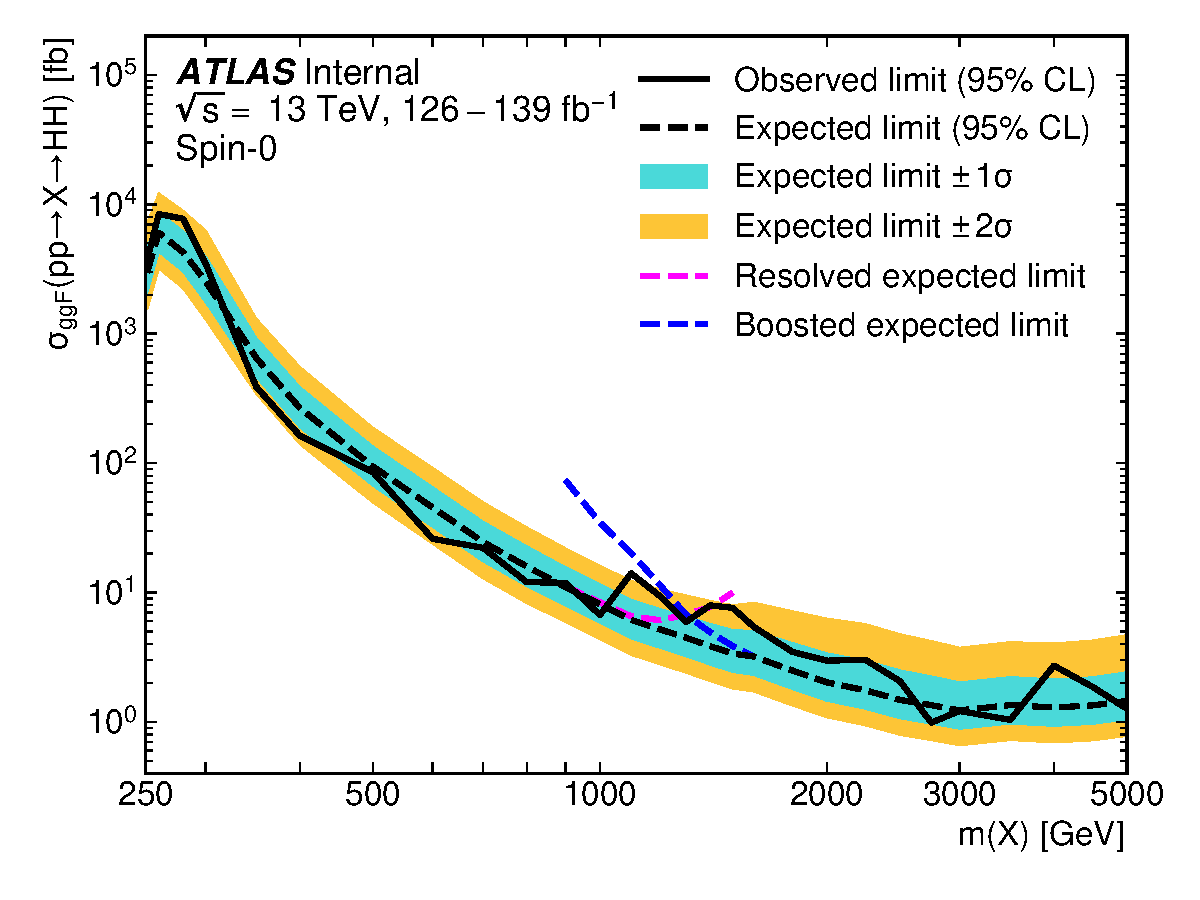
\includegraphics[width=0.65\textwidth]{figures/limits-scalar-5-TeV.pdf}
  }

  \subfloat[]{
    \label{fig:limits-spin2}
    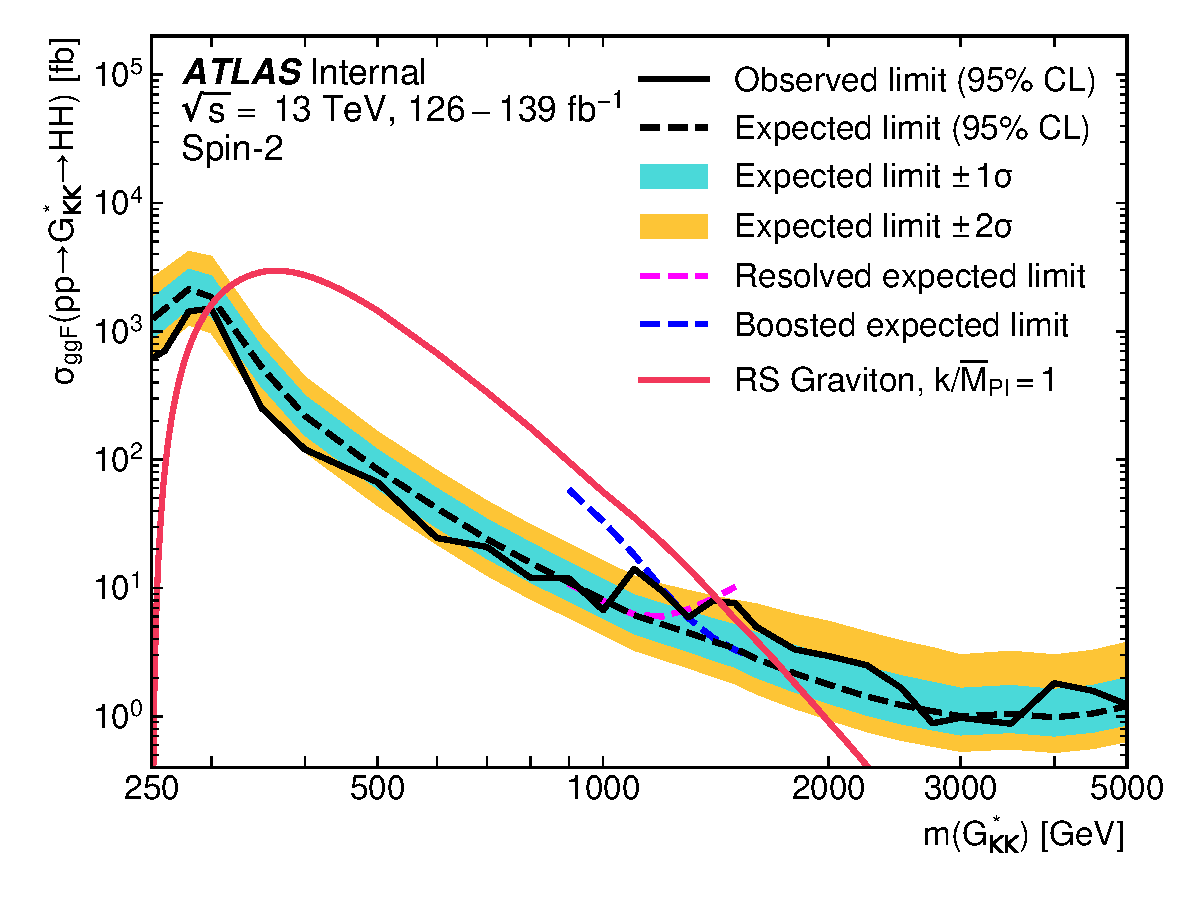
\includegraphics[width=0.65\textwidth]{figures/limits-graviton-5-TeV.pdf}
  }
  \caption{\label{fig:res-limits}
    Expected (dashed black) and observed (solid black) 95\% CL upper limits on the cross-section times branching ratio of resonant production for spin-0 (\(X \rightarrow HH\)) and spin-2 (\(G_{KK}^{*} \rightarrow HH\)). 
    The \(\pm 1\sigma\) and \(\pm 2\sigma\) ranges for the expected limits are shown in the colored bands. 
    The resolved channel expected limit is shown in dashed pink and covers the range from \SIlist{251;1500}{\GeV}. 
    It is combined with the boosted channel (dashed blue) between \SIlist{900;1500}{\GeV}.
    The theoretical prediction for the bulk RS model with \(k/\overline{M}_{\mathrm{Pl}} = 1\)~\cite{Carvalho} 
    (solid red line) is shown, with the decrease below \SI{350}{\GeV} due to a sharp reduction in the \(G_{KK}^{*} \rightarrow HH\) branching ratio. The nominal \(H \rightarrow b\bar{b}\) branching ratio is taken as 0.582. Note 
    that all results use the asymptotic approximation, though the validity of this approximation for the boosted results 
    above \SI{3}{\TeV} is being evaluated.}
\end{figure}

\begin{figure}[ht]
  \centering
  \vspace*{-3cm}
  \subfloat[]{
    \label{fig:limits-spin0-early-Run2}
    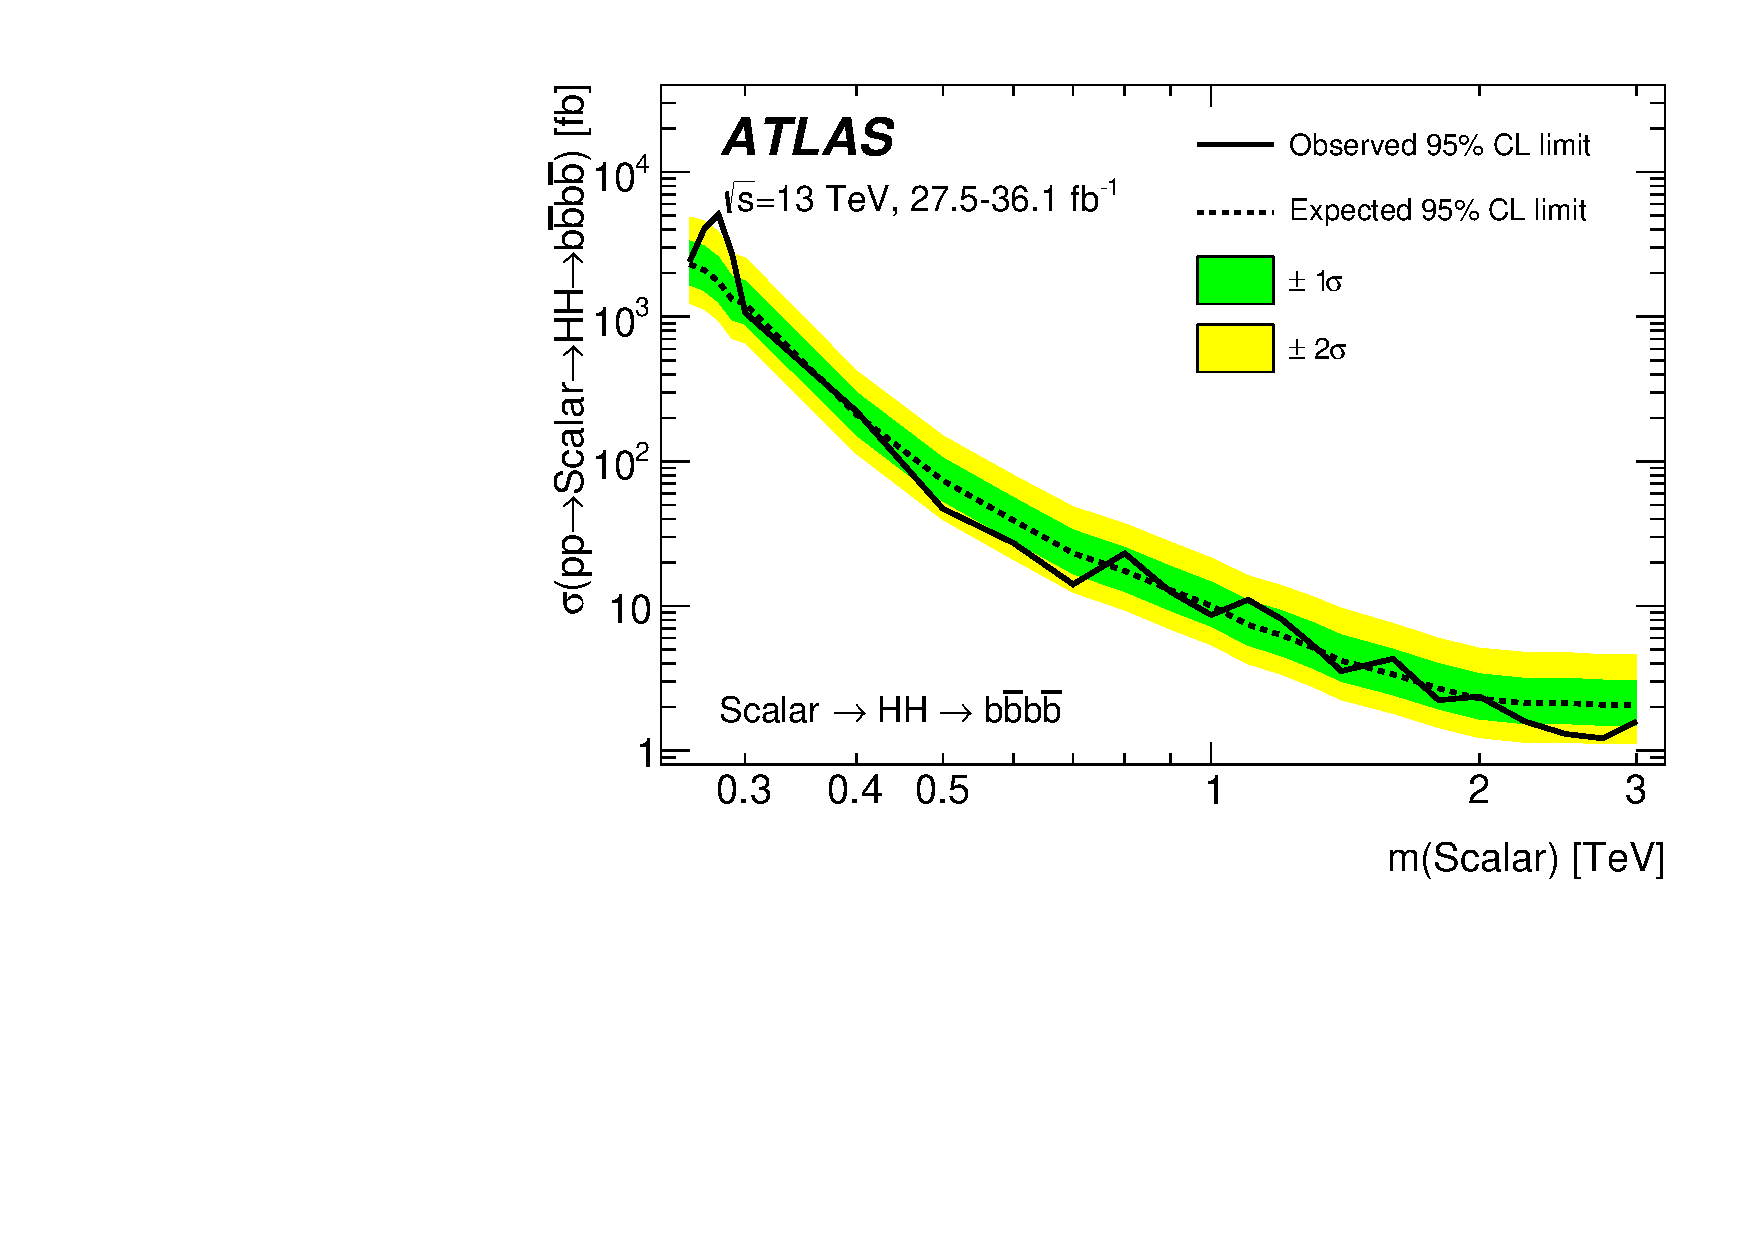
\includegraphics[width=0.65\textwidth]{figures/scalar-limits-early-Run2.pdf}
  }

  \subfloat[]{
    \label{fig:limits-spin2-early-Run-2}
    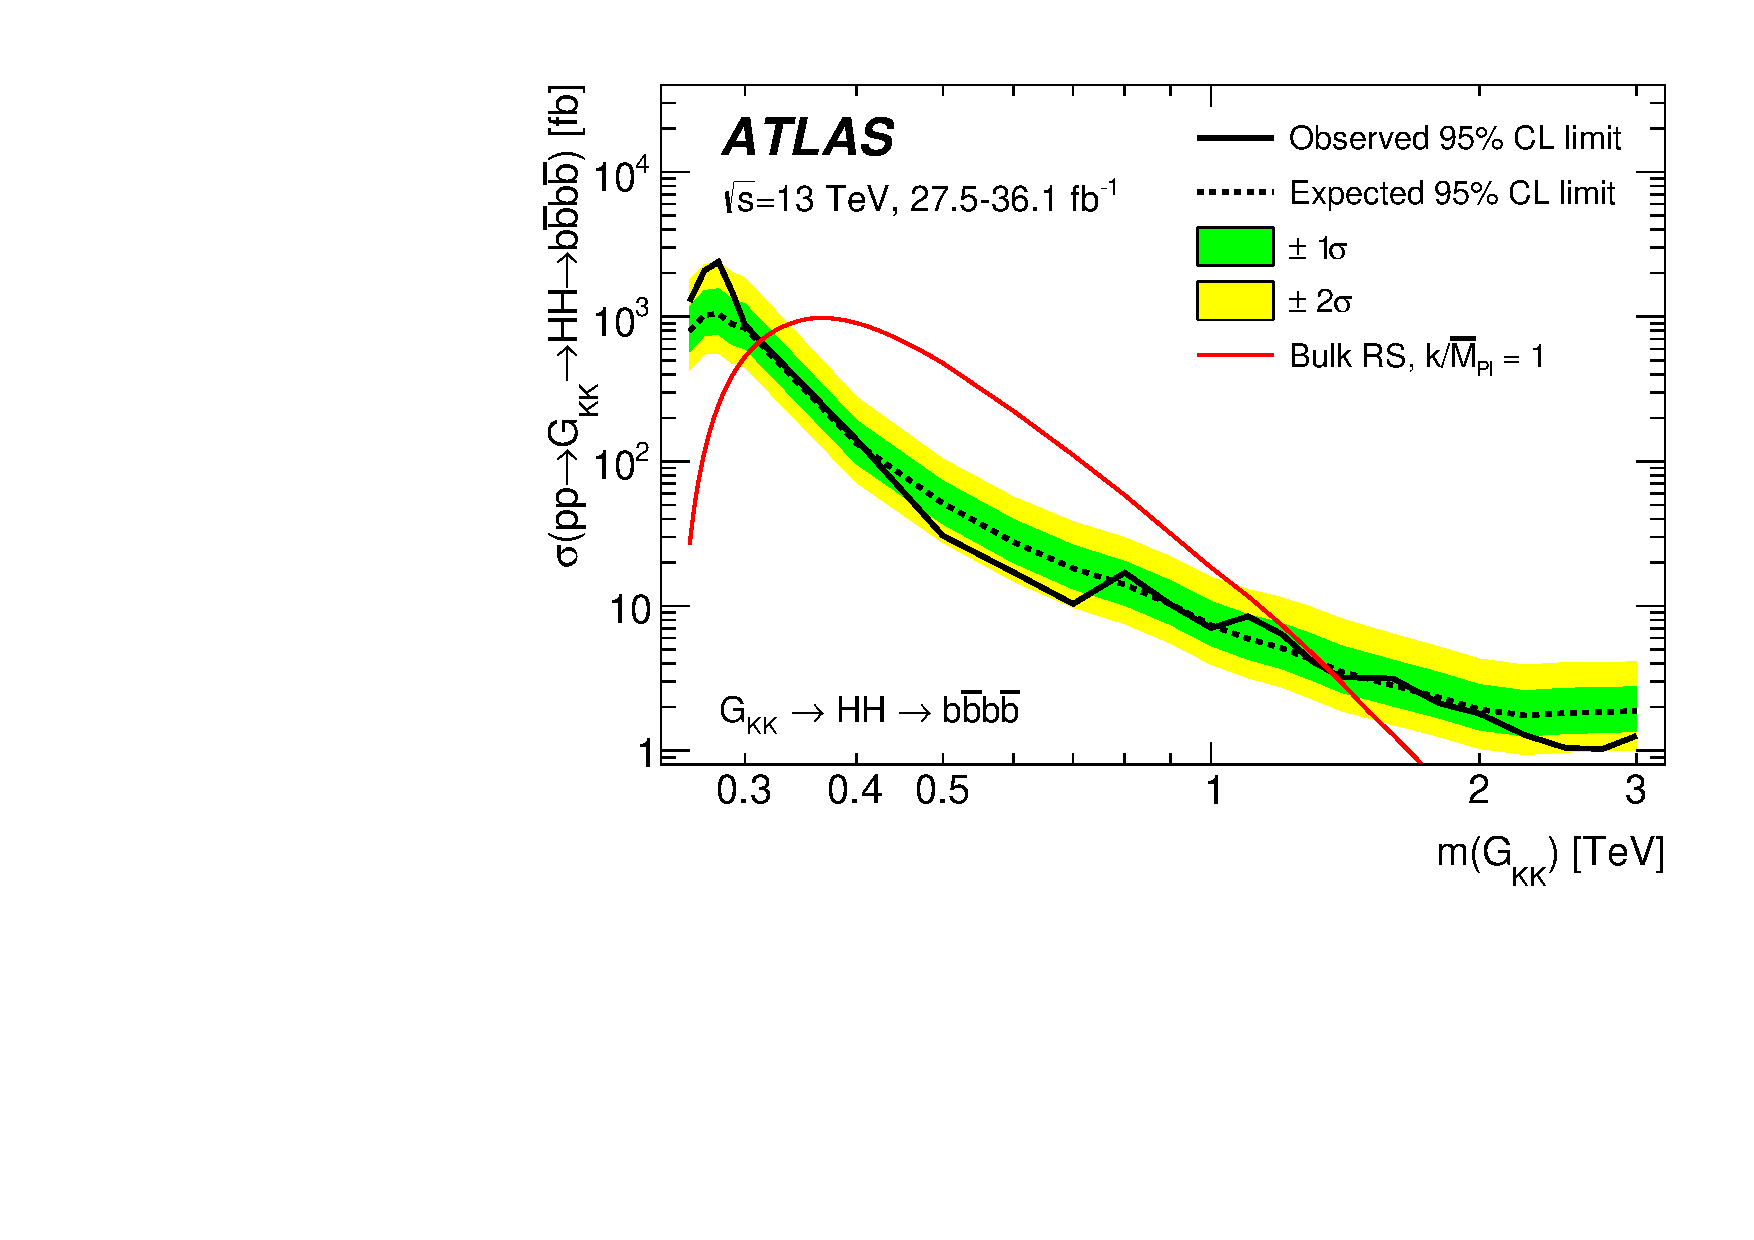
\includegraphics[width=0.65\textwidth]{figures/grav-limits-early-Run2.pdf}
  }
  \caption{\label{fig:res-limits-early-Run-2} Expected (dashed black) and observed (solid black) 95\% CL upper limits 
  or spin-0 (Scalar\(\rightarrow HH\rightarrow \bbbb \)) and spin-2 (\(G_{KK} \rightarrow HH \rightarrow \bbbb\)) from the
  early Run 2 $4b$ search~\cite{EXOT-2016-31}, to be compared with the results in Figure \ref{fig:res-limits}. Note that 
  the $y$-axis scaling differs from Figure \ref{fig:res-limits} by a factor of the $HH\rightarrow \bbbb$ branching ratio.
  An excess is present at \SI{280}{\GeV}, with local (global) significance $3.6 (2.3)\sigma$. The spin-2 
  bulk Randall-Sundrum model with $k/\overline{M}_{\mathrm{Pl}} = 1$ is excluded for graviton masses between \SIlist{313;1362}{\GeV}.}
\end{figure}

Results from the early Run 2 $4b$ resonant search~\cite{EXOT-2016-31} are included in Figure 
\ref{fig:res-limits-early-Run-2} for comparison. The full Run 2 results of this thesis represent an 
improvement in sensitivity, 
with an expanded exclusion for the spin-2 search of graviton masses between \SIlist{298;1440}{\GeV}, relative 
to the early Run 2 result, 
with exclusion between \SIlist{313;1362}{\GeV}. An excess is present in the early Run 2 results at \SI{280}{\GeV}, 
with local (global) significance $3.6 (2.3)\sigma$. This is no longer present in the full Run 2 results, 
indicative of improved background modeling in this low mass region.

Preliminary results are presented here for the gluon-gluon fusion non-resonant search, combining results from the $4b$ 
and $3b+1l$ signal regions in the $2\times 2$ category scheme in $\Delta \eta_{HH}$ and $X_{HH}$. These results will be 
further combined with a VBF channel (discussed in Appendix \ref{app:other-channels}), but this is left for future work. 
Results shown here include 
background all background uncertainties, but do not include signal systematics. Limits are set for $\kappa_{\lambda}$ 
values from $-20$ to $20$. 
The cross section limit for $HH$ production is set at \SI{140}{\fb} (\SI{180}{\fb}) observed (expected), 
corresponding to an observed (expected) limit of $4.4$ ($5.9$) times the Standard Model prediction 
(see Table \ref{tbl:SM-HH-limits}). 
$\kappa_{\lambda}$ is constrained to be within the range $-4.9 \leq \kappa_{\lambda} \leq 14.4$ observed 
($-3.9 \leq \kappa_{\lambda} \leq 10.9$ expected). These results are shown in Figure \ref{fig:nonres-limits}.

\begin{table}
\centering
\begin{tabular}{ |c|c|c|c|c|c| } 
\hline
\textbf{Observed} & $-2\sigma$ & $-1\sigma$ & \textbf{Expected} & $+1\sigma$ & $+2\sigma$\\
 \hline
\textbf{4.4}	& 3.1	& 4.2 & \textbf{5.9}	& 8.2 & 11.0\\
 \hline
\end{tabular}
 \caption{\label{tbl:SM-HH-limits} Limits on Standard Model $HH\rightarrow \bbbb$ production, presented in units of the 
predicted Standard Model cross section. Results do not include signal systematics.}
\end{table}

This is a significant improvement over the early Run 2 result, which achieved an observed (expected) 
limit of 12.9 (20.7) times the Standard Model prediction. The dataset is 4.6 times larger, and a naive scaling 
of the early Run 2 result (Poisson statistics $\implies$ a factor of $1/\sqrt{4.6}$) would predict an observed (expected)
limit of 6.0 (9.7) times the Standard Model. The result of 4.4 (5.9) observed (expected) presented here is 
therefore both an improvement by a factor of 3 (3.5) over the previous result and also beats the statistical 
scaling by around 30 (40)~\%, demonstrating the impact of the various analysis improvements presented here. Note again that these results do not include the complete set of uncertainties -- however, the addition 
of the remaining uncertainties is expected to have no more than a few percent impact.

Further comparisons of both the resonant and non-resonant results are presented in Chapter \ref{chap:compare}.

\begin{figure}[ht]
  \centering
  \subfloat{
    \label{fig:limits-kl}
    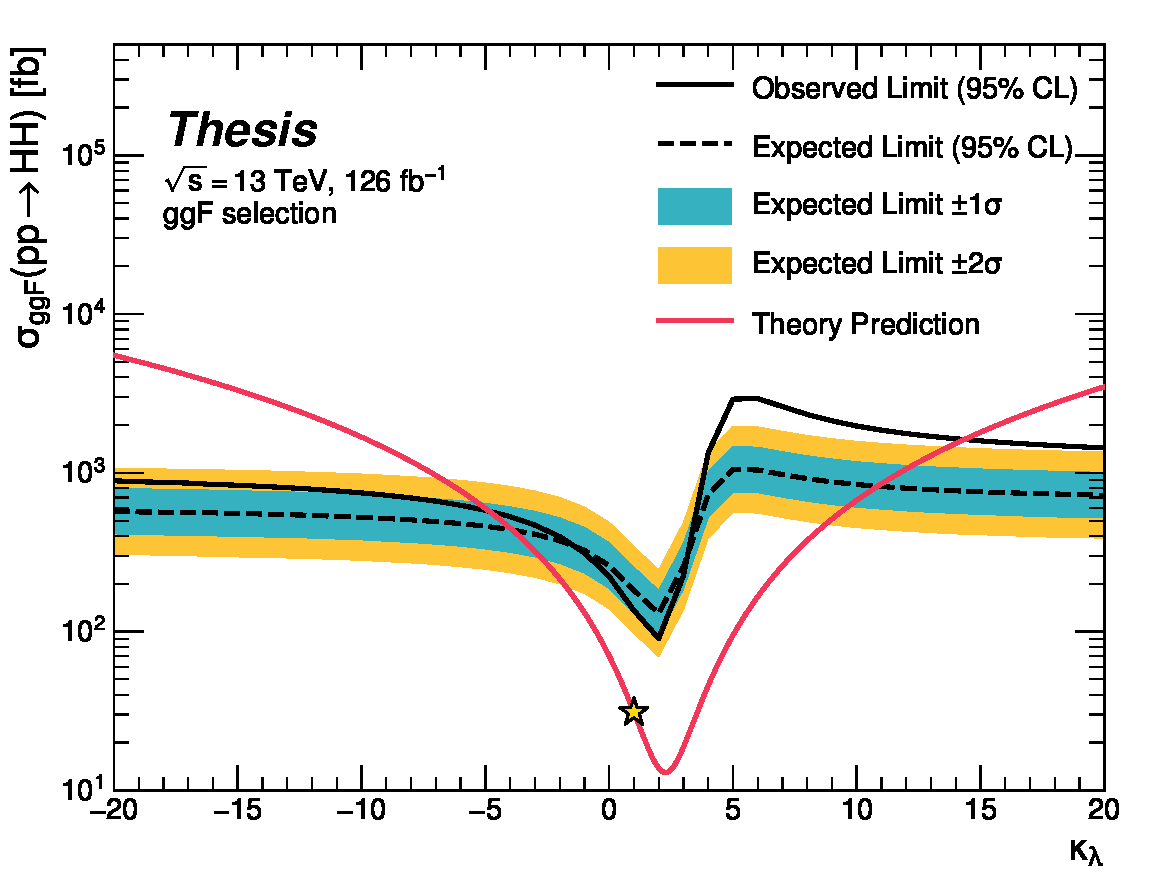
\includegraphics[width=0.8\textwidth]{figures/obs-limit-2x2.pdf}
  }
  \caption{\label{fig:nonres-limits}
    Expected (dashed black) and observed (solid black) 95\% CL upper limits on the cross-section times 
    branching ratio of non-resonant production 
    for a range of values of the Higgs self-coupling, with the Standard Model value ($\kappa_{\lambda} = 1$) illustrated 
    with a star. The \(\pm 1\sigma\) and \(\pm 2\sigma\) ranges for the expected limits are shown in the colored bands. 
    The cross section limit for $HH$ production is set at \SI{140}{\fb} (\SI{180}{\fb}) observed (expected), 
    corresponding to an observed (expected) limit of $4.4$ ($5.9$) times the Standard Model prediction. 
    $\kappa_{\lambda}$ is constrained to be within the range $-4.9 \leq \kappa_{\lambda} \leq 14.4$ observed 
    ($-3.9 \leq \kappa_{\lambda} \leq 10.9$ expected). The nominal \(H \rightarrow b\bar{b}\) branching ratio is 
    taken as 0.582. The excess present for $\kappa_{\lambda}\geq 5$ is thought to be due to a low mass 
    background mis-modeling, present due to the optimization of this analysis for the Standard Model point, and is not present in more sensitive channels in this same region (e.g. $HH\rightarrow bb\gamma\gamma$~\cite{ATLAS-CONF-2021-016}).
  }
\end{figure}

The observed limits presented in Figure \ref{fig:nonres-limits} are consistently above the $2\sigma$ band for values of 
$\kappa_{\lambda} \geq 5$, peaking at a local significance of $3.8\sigma$ for $\kappa_{\lambda} = 6$. 
As this analysis is optimized for points near the Standard Model, and as there is no excess present in more 
sensitive channels in this same region (e.g. $HH\rightarrow bb\gamma\gamma$~\cite{ATLAS-CONF-2021-016}), it is 
not believed this is a real effect, but is rather due to a mis-modeling of the background at low mass, where 
the $\min{\Delta R}$ pairing 
has poor signal efficiency and the assumption of well behaved background in the mass plane breaks down. This is 
consistent with the location of the $\kappa_{\lambda} = 6$ signal in $m_{HH}$, as shown in Figures \ref{fig:nonres-sr-mhh-4b} and \ref{fig:nonres-sr-mhh-3b1l}.
It was considered, but not implemented, for this analysis to impose a cut on $m_{HH}$ near $350$ or \SI{400}{\GeV} to avoid such a low mass modeling issue.

To check the impact of if such a cut would have been imposed, and to verify that the excess is due to the low mass regime, 
the same set of limits is run without the low mass bins. In this case, the first few bins in $m_{HH}$ are simply dropped, 
such that everything else, including the higher mass bin edges, is kept the same. Due to 
the variable width binning, this corresponds to an $m_{HH}$ cut of \SI{381}{\GeV}. The results of this check are shown 
in Figure \ref{fig:nonres-limits-with-cut}, and the corresponding limits for Standard Model $HH$ are 
quoted in Table \ref{tbl:SM-HH-limits-mhh-cut}.
With the $m_{HH}$ cut imposed, there is a slight degradation in the expected limits for larger positive and negative 
values of $\kappa_{\lambda}$, but the points near the Standard Model are nearly identical. Further, the observed excess 
is significantly reduced, with observed limits for $\kappa_{\lambda} \geq 5$ now falling entirely within the expected 
$1\sigma$ band. Due to the preliminary nature of these results, further study is left for future work. However, 
in conjunction with the $HH\rightarrow bb\gamma\gamma$ results and expectations about the difficulty 
of the background estimation at low mass, it is believed that this is demonstrative of a mis-modeling rather than a real excess. 

\begin{figure}[ht]
  \centering
  \subfloat{
    \label{fig:limits-kl-with-cut}
    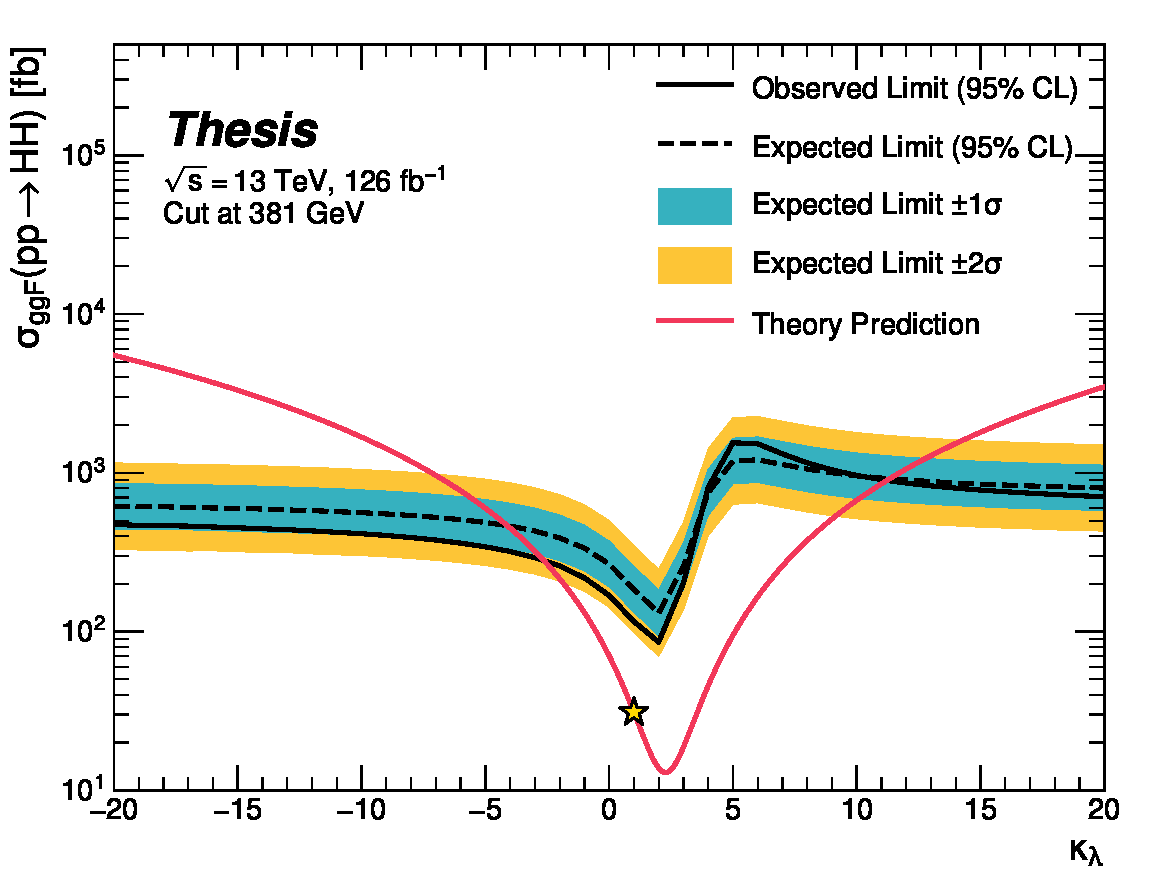
\includegraphics[width=0.8\textwidth]{figures/obs-limit-2x2-cut-at-381-only.pdf}
  }
  \caption{\label{fig:nonres-limits-with-cut} Limits including only events above \SI{381}{\GeV} in $m_{HH}$, 
  to be compared with the limits in Figure \ref{fig:nonres-limits}. Such a cut is accomplished by 
  dropping $m_{HH}$ bins below \SI{381}{\GeV}, with the value 
  of \SI{381}{\GeV} determined by the optimized variable width binning. All other aspects of the procedure 
  and inputs are kept the same as in Figure \ref{fig:nonres-limits}. The excess 
  at and above $\kappa_{\lambda} = 5$ is significantly reduced, demonstrating that such an excess is driven by 
  low mass. Notably, there is minimal impact on the expected sensitivity with this $m_{HH}$ cut.
  }
\end{figure}

\begin{table}
\centering
\begin{tabular}{ |c|c|c|c|c|c| } 
\hline
\textbf{Observed} & $-2\sigma$ & $-1\sigma$ & \textbf{Expected} & $+1\sigma$ & $+2\sigma$\\
 \hline
\textbf{3.7}	& 3.2	& 4.3 & \textbf{5.9}	& 8.3 & 11.2\\
 \hline
\end{tabular}
 \caption{\label{tbl:SM-HH-limits-mhh-cut} Limits on Standard Model $HH\rightarrow \bbbb$ production, 
 presented in units of the predicted Standard Model cross section, corresponding to the $m_{HH} > \SI{381}{\GeV}$ 
 selection of Figure \ref{fig:nonres-limits-with-cut}. Results do not include signal systematics. The deficit 
 in the observed limit is larger than that of Table \ref{tbl:SM-HH-limits}, but still within the $2\sigma$ band. There 
 are only very minor differences in the expected limit band.}
\end{table}
